% Options for packages loaded elsewhere
\PassOptionsToPackage{unicode}{hyperref}
\PassOptionsToPackage{hyphens}{url}
\PassOptionsToPackage{dvipsnames,svgnames*,x11names*}{xcolor}
%
\documentclass[
]{krantz}
\usepackage{lmodern}
\usepackage{amssymb,amsmath}
\usepackage{ifxetex,ifluatex}
\ifnum 0\ifxetex 1\fi\ifluatex 1\fi=0 % if pdftex
  \usepackage[T1]{fontenc}
  \usepackage[utf8]{inputenc}
  \usepackage{textcomp} % provide euro and other symbols
\else % if luatex or xetex
  \usepackage{unicode-math}
  \defaultfontfeatures{Scale=MatchLowercase}
  \defaultfontfeatures[\rmfamily]{Ligatures=TeX,Scale=1}
\fi
% Use upquote if available, for straight quotes in verbatim environments
\IfFileExists{upquote.sty}{\usepackage{upquote}}{}
\IfFileExists{microtype.sty}{% use microtype if available
  \usepackage[]{microtype}
  \UseMicrotypeSet[protrusion]{basicmath} % disable protrusion for tt fonts
}{}
\makeatletter
\@ifundefined{KOMAClassName}{% if non-KOMA class
  \IfFileExists{parskip.sty}{%
    \usepackage{parskip}
  }{% else
    \setlength{\parindent}{0pt}
    \setlength{\parskip}{6pt plus 2pt minus 1pt}}
}{% if KOMA class
  \KOMAoptions{parskip=half}}
\makeatother
\usepackage{xcolor}
\IfFileExists{xurl.sty}{\usepackage{xurl}}{} % add URL line breaks if available
\IfFileExists{bookmark.sty}{\usepackage{bookmark}}{\usepackage{hyperref}}
\hypersetup{
  pdftitle={Broadening Your Statistical Horizons},
  pdfauthor={Paul Roback and Julie Legler},
  colorlinks=true,
  linkcolor=Maroon,
  filecolor=Maroon,
  citecolor=Blue,
  urlcolor=Blue,
  pdfcreator={LaTeX via pandoc}}
\urlstyle{same} % disable monospaced font for URLs
\usepackage{color}
\usepackage{fancyvrb}
\newcommand{\VerbBar}{|}
\newcommand{\VERB}{\Verb[commandchars=\\\{\}]}
\DefineVerbatimEnvironment{Highlighting}{Verbatim}{commandchars=\\\{\}}
% Add ',fontsize=\small' for more characters per line
\usepackage{framed}
\definecolor{shadecolor}{RGB}{248,248,248}
\newenvironment{Shaded}{\begin{snugshade}}{\end{snugshade}}
\newcommand{\AlertTok}[1]{\textcolor[rgb]{0.33,0.33,0.33}{#1}}
\newcommand{\AnnotationTok}[1]{\textcolor[rgb]{0.37,0.37,0.37}{\textbf{\textit{#1}}}}
\newcommand{\AttributeTok}[1]{\textcolor[rgb]{0.61,0.61,0.61}{#1}}
\newcommand{\BaseNTok}[1]{\textcolor[rgb]{0.06,0.06,0.06}{#1}}
\newcommand{\BuiltInTok}[1]{#1}
\newcommand{\CharTok}[1]{\textcolor[rgb]{0.5,0.5,0.5}{#1}}
\newcommand{\CommentTok}[1]{\textcolor[rgb]{0.37,0.37,0.37}{\textit{#1}}}
\newcommand{\CommentVarTok}[1]{\textcolor[rgb]{0.37,0.37,0.37}{\textbf{\textit{#1}}}}
\newcommand{\ConstantTok}[1]{\textcolor[rgb]{0,0,0}{#1}}
\newcommand{\ControlFlowTok}[1]{\textcolor[rgb]{0.27,0.27,0.27}{\textbf{#1}}}
\newcommand{\DataTypeTok}[1]{\textcolor[rgb]{0.27,0.27,0.27}{#1}}
\newcommand{\DecValTok}[1]{\textcolor[rgb]{0.06,0.06,0.06}{#1}}
\newcommand{\DocumentationTok}[1]{\textcolor[rgb]{0.37,0.37,0.37}{\textbf{\textit{#1}}}}
\newcommand{\ErrorTok}[1]{\textcolor[rgb]{0.14,0.14,0.14}{\textbf{#1}}}
\newcommand{\ExtensionTok}[1]{#1}
\newcommand{\FloatTok}[1]{\textcolor[rgb]{0.06,0.06,0.06}{#1}}
\newcommand{\FunctionTok}[1]{\textcolor[rgb]{0,0,0}{#1}}
\newcommand{\ImportTok}[1]{#1}
\newcommand{\InformationTok}[1]{\textcolor[rgb]{0.37,0.37,0.37}{\textbf{\textit{#1}}}}
\newcommand{\KeywordTok}[1]{\textcolor[rgb]{0.27,0.27,0.27}{\textbf{#1}}}
\newcommand{\NormalTok}[1]{#1}
\newcommand{\OperatorTok}[1]{\textcolor[rgb]{0.43,0.43,0.43}{\textbf{#1}}}
\newcommand{\OtherTok}[1]{\textcolor[rgb]{0.37,0.37,0.37}{#1}}
\newcommand{\PreprocessorTok}[1]{\textcolor[rgb]{0.37,0.37,0.37}{\textit{#1}}}
\newcommand{\RegionMarkerTok}[1]{#1}
\newcommand{\SpecialCharTok}[1]{\textcolor[rgb]{0,0,0}{#1}}
\newcommand{\SpecialStringTok}[1]{\textcolor[rgb]{0.5,0.5,0.5}{#1}}
\newcommand{\StringTok}[1]{\textcolor[rgb]{0.5,0.5,0.5}{#1}}
\newcommand{\VariableTok}[1]{\textcolor[rgb]{0,0,0}{#1}}
\newcommand{\VerbatimStringTok}[1]{\textcolor[rgb]{0.5,0.5,0.5}{#1}}
\newcommand{\WarningTok}[1]{\textcolor[rgb]{0.37,0.37,0.37}{\textbf{\textit{#1}}}}
\usepackage{longtable,booktabs}
% Correct order of tables after \paragraph or \subparagraph
\usepackage{etoolbox}
\makeatletter
\patchcmd\longtable{\par}{\if@noskipsec\mbox{}\fi\par}{}{}
\makeatother
% Allow footnotes in longtable head/foot
\IfFileExists{footnotehyper.sty}{\usepackage{footnotehyper}}{\usepackage{footnote}}
\makesavenoteenv{longtable}
\usepackage{graphicx,grffile}
\makeatletter
\def\maxwidth{\ifdim\Gin@nat@width>\linewidth\linewidth\else\Gin@nat@width\fi}
\def\maxheight{\ifdim\Gin@nat@height>\textheight\textheight\else\Gin@nat@height\fi}
\makeatother
% Scale images if necessary, so that they will not overflow the page
% margins by default, and it is still possible to overwrite the defaults
% using explicit options in \includegraphics[width, height, ...]{}
\setkeys{Gin}{width=\maxwidth,height=\maxheight,keepaspectratio}
% Set default figure placement to htbp
\makeatletter
\def\fps@figure{htbp}
\makeatother
\setlength{\emergencystretch}{3em} % prevent overfull lines
\providecommand{\tightlist}{%
  \setlength{\itemsep}{0pt}\setlength{\parskip}{0pt}}
\setcounter{secnumdepth}{5}
\usepackage{booktabs}
%These packages added to resolve tex problems arising from kable tables.
\usepackage{tabularx}
\usepackage{float}
%%
\usepackage{longtable}
\usepackage[bf,singlelinecheck=off]{caption}

\usepackage{framed,color}
\definecolor{shadecolor}{RGB}{248,248,248}

\renewcommand{\textfraction}{0.05}
\renewcommand{\topfraction}{0.8}
\renewcommand{\bottomfraction}{0.8}
\renewcommand{\floatpagefraction}{0.75}

%%%%%%%%
% Inserting new commands here

%% Chapter 2
\newcommand{\lik}{\mathrm{Lik}}
\newcommand{\Lik}{\mathrm{Lik}}

\newcommand{\bstop}{p_{S|B1}}
\newcommand{\nstop}{p_{S|N}}

\newcommand{\thisismynewcommand}{p_{B|\textrm{B Bias}}}
\newcommand{\neutral}{p_{B|N}}
\newcommand{\gbias}{p_{B|\textrm{G Bias}}}
\newcommand{\bbias}{p_{B|\textrm{B Bias}}}

%% Chapter 3
\newcommand{\E}{\operatorname{E}}
\newcommand{\SD}{\operatorname{SD}}

%% Chapter 5
\newcommand{\var}{\operatorname{Var}}

%%%%%%%%

\renewenvironment{quote}{\begin{VF}}{\end{VF}}
\let\oldhref\href
\renewcommand{\href}[2]{#2\footnote{\url{#1}}}

\makeatletter
\newenvironment{kframe}{%
\medskip{}
\setlength{\fboxsep}{.8em}
 \def\at@end@of@kframe{}%
 \ifinner\ifhmode%
  \def\at@end@of@kframe{\end{minipage}}%
  \begin{minipage}{\columnwidth}%
 \fi\fi%
 \def\FrameCommand##1{\hskip\@totalleftmargin \hskip-\fboxsep
 \colorbox{shadecolor}{##1}\hskip-\fboxsep
     % There is no \\@totalrightmargin, so:
     \hskip-\linewidth \hskip-\@totalleftmargin \hskip\columnwidth}%
 \MakeFramed {\advance\hsize-\width
   \@totalleftmargin\z@ \linewidth\hsize
   \@setminipage}}%
 {\par\unskip\endMakeFramed%
 \at@end@of@kframe}
\makeatother

% This change to the shaded environment adapted from https://github.com/yihui/bookdown-chinese/commit/a3e392593b464ba31a7eceb0cd60f7e0bd112798 and https://stackoverflow.com/questions/41052687/rstudio-pdf-knit-fails-with-environment-shaded-undefined-error
\makeatletter
\@ifundefined{Shaded}{
}{\renewenvironment{Shaded}{\begin{kframe}}{\end{kframe}}}
\makeatother

\usepackage{makeidx}
\makeindex

\urlstyle{tt}

\usepackage{amsthm}
\makeatletter
\def\thm@space@setup{%
  \thm@preskip=8pt plus 2pt minus 4pt
  \thm@postskip=\thm@preskip
}
\makeatother

\frontmatter
\usepackage[]{natbib}
\bibliographystyle{plainnat}

\title{Broadening Your Statistical Horizons}
\usepackage{etoolbox}
\makeatletter
\providecommand{\subtitle}[1]{% add subtitle to \maketitle
  \apptocmd{\@title}{\par {\large #1 \par}}{}{}
}
\makeatother
\subtitle{Generalized Linear Models and Multilevel Models}
\author{Paul Roback and Julie Legler}
\date{2020-06-01}

\begin{document}
\maketitle

% you may need to leave a few empty pages before the dedication page

%\cleardoublepage\newpage\thispagestyle{empty}\null
%\cleardoublepage\newpage\thispagestyle{empty}\null
%\cleardoublepage\newpage
\thispagestyle{empty}

\setlength{\abovedisplayskip}{-5pt}
\setlength{\abovedisplayshortskip}{-5pt}

{
\hypersetup{linkcolor=}
\setcounter{tocdepth}{2}
\tableofcontents
}
\hypertarget{preface}{%
\chapter*{Preface}\label{preface}}


Placeholder

\hypertarget{ch-MLRreview}{%
\chapter{Review of Multiple Linear Regression}\label{ch-MLRreview}}

\hypertarget{learning-objectives}{%
\section{Learning Objectives}\label{learning-objectives}}

After finishing this chapter, you should be able to:

\begin{itemize}
\tightlist
\item
  Identify cases where ordinary least squares (OLS) assumptions are violated.
\item
  Generate exploratory data analysis plots and summary statistics.
\item
  Use residual diagnostics to examine OLS assumptions.
\item
  Interpret parameters and associated tests and intervals from multiple regression models.
\item
  Understand the basic ideas behind bootstrapped confidence intervals.
\end{itemize}

\hypertarget{introduction-to-broadening-your-statistical-horizons}{%
\section{Introduction to Broadening Your Statistical Horizons}\label{introduction-to-broadening-your-statistical-horizons}}

Ecologists count species, criminologists count arrests, and cancer specialists count cases. Political scientists seek to explain who is a Democrat, pre-med students are curious about who gets in to medical school, and sociologists study which people get tattoos. In the first case, ecologists, criminologists and cancer specialists are concerned about outcomes which are counts. The political scientists', pre-med students' and sociologists' interest centers on binary responses: Democrat or not, accepted or not, and tattooed or not. We can model these non-Gaussian (non-normal) responses in a more natural way by fitting \textbf{generalized linear models (GLMs)} as opposed to using to \textbf{linear least squares regression} models.

When models are fit to data using OLS, inferences are possible using traditional statistical theory under certain conditions: if we can assume that there is a linear relationship between the response (Y) and an explanatory variable (X), the observations are independent of one another, the responses are approximately normal for each level of the X, and the variation in the responses is the same for each level of X. If we intend to make inferences using GLMs, necessary assumptions are different. First, we will not be constrained by the normality assumption. When conditions are met, GLMs can accommodate non-normal responses such as the counts and binary data in our preceding examples. While the observations must still be independent of one another, the variance in Y at each level of X need not be equal nor does the assumption of linearity between Y and X need to be plausible.

However GLMs cannot be used for models in the following circumstances: medical researchers collect data on patients in clinical trials weekly for 6 months; rat dams are injected with teratogenic substances and their offspring are monitored for defects; and, musicians' performance anxiety is recorded for several performances. Each of these examples involves correlated data: the same patient's outcomes are more likely to be similar from week-to-week than outcomes from different patients; litter mates are more likely to suffer defects at similar rates in contrast to unrelated rat pups; and, a musician's anxiety is more similar from performance to performance than it is with other musicians. Each of these examples violate the independence assumption of simpler linear models for OLS or GLM inference.

The \textbf{Generalized Linear Models} in the book's title extends OLS methods you may have seen in linear regression to handle responses that are non-normal. The \textbf{Multilevel Methods} will allow us to create models for situations where the observations are not independent of one another. Overall, these approaches will permit us to get much more out of data and may be more faithful to the actual data structure than models based on ordinary least squares. These models will \emph{broaden your statistical horizons}.

In order to understand the motivation for handling violations of assumptions, it is helpful to be able to recognize the model assumptions for inference with OLS in the context of different studies. While linearity is sufficient for fitting an OLS model, in order to make inferences and predictions the observations must also be independent, the responses should be approximately normal at each level of the predictors, and the standard deviation of the responses at each level of the predictors should be approximately equal. After examining circumstances where inference with OLS modeling is appropriate, we will look for violations of these assumptions in other sets of circumstances. These are settings where we may be able to use the methods of this text. We've kept the examples in the exposition simple to fix ideas. There are exercises which describe more realistic and complex studies.

\hypertarget{ordinary-least-squares-ols-assumptions}{%
\section{Ordinary Least Squares (OLS) Assumptions}\label{ordinary-least-squares-ols-assumptions}}

\begin{figure}

{\centering 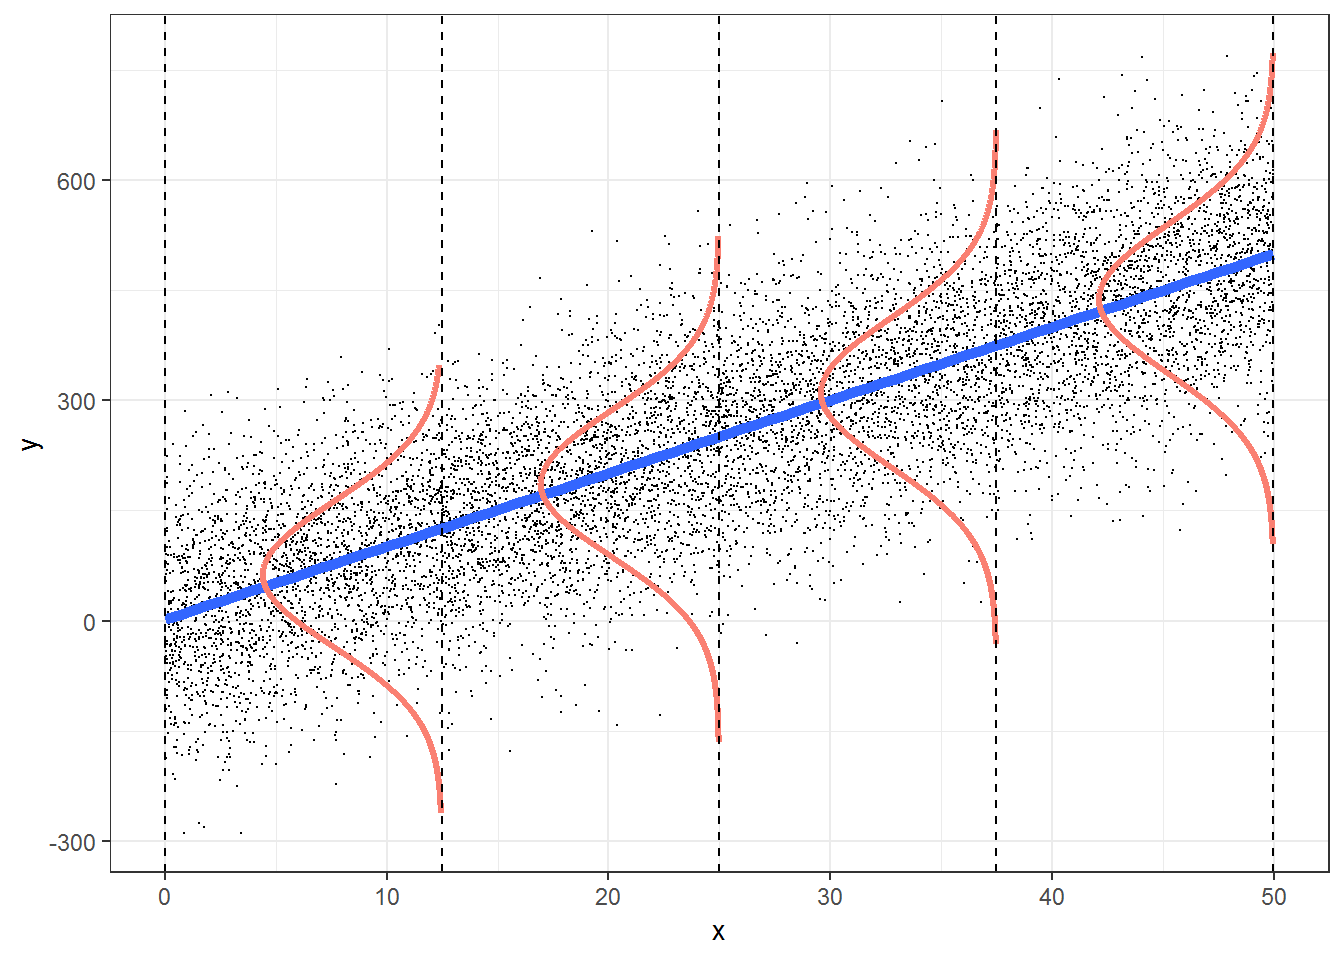
\includegraphics[width=0.9\linewidth]{bookdown-bysh_files/figure-latex/OLSassumptions-1} 

}

\caption{Ordinary least squares assumptions}\label{fig:OLSassumptions}
\end{figure}

Recall that making inferences or predictions with models fit using ordinary least squares (OLS) requires that the following assumptions be tenable. The acronym LINE can be used to recall the assumptions required for making inferences and predictions with models based on OLS. If we consider a simple linear regression with just a single predictor X, then:

\begin{itemize}
\tightlist
\item
  \textbf{L:} there is a linear relationship between the mean response (Y) and the explanatory variable (X),
\item
  \textbf{I:} the errors are independent---there's no connection between how far any two points lie from the regression line,
\item
  \textbf{N:} the responses are normally distributed at each level of X, and
\item
  \textbf{E:} the variance or, equivalently, the standard deviation of the responses is equal for all levels of X.
\end{itemize}

These assumptions are depicted in Figure \ref{fig:OLSassumptions}.

\begin{itemize}
\tightlist
\item
  \textbf{L:} The mean value for Y at each level of X falls on the regression line.
\item
  \textbf{I:} We'll need to check the design of the study to determine if the errors (vertical distances from the line) are independent of one another.
\item
  \textbf{N:} At each level of X, the values for Y are normally distributed.
\item
  \textbf{E:} The spread in the Y's for each level of X is the same.
\end{itemize}

\hypertarget{cases-that-do-not-violate-the-ols-assumptions-for-inference}{%
\subsection{Cases that do not violate the OLS assumptions for inference}\label{cases-that-do-not-violate-the-ols-assumptions-for-inference}}

It can be argued that the following studies do not violate the OLS assumptions for inference. We begin by identifying the response and the explanatory variables followed by describing each of the LINE assumptions in the context of the study, commenting on possible problems with the assumptions.

\begin{enumerate}
\def\labelenumi{\arabic{enumi})}
\item
  \textbf{Reaction times and car radios.} A researcher suspects that loud music can affect how quickly drivers react. She randomly selects drivers to drive the same stretch of road with varying levels of music volume. Stopping distances for each driver are measured along with the decibel level of the music on their car radio.

  \begin{itemize}
  \tightlist
  \item
    \emph{Response variable:} Reaction time
  \item
    \emph{Explanatory variable:} Decibel level of music\\
  \end{itemize}

  The OLS assumptions for inference would apply if:

  \begin{itemize}
  \tightlist
  \item
    \textbf{L:} The mean reaction time is linearly related to decibel level of the music.
  \item
    \textbf{I:} Stopping distances are independent. The random selection of drivers should assure independence.
  \item
    \textbf{N:} The stopping distances for a given decibel level of music vary and are normally distributed.
  \item
    \textbf{E:} The variation in stopping distances should be approximately the same for each decibel level of music.\\
  \end{itemize}

  There are potential problems with the linearity and equal standard deviation assumptions. For example, if there is threshold for the volume of music where the effect on reaction times remains the same, mean reaction times would not be a linear function of music. Another problem may occur if a few subjects at each decibel level took a really long time to react. In this case, reaction times would be right skewed and the normality assumption would be violated. Often we can think of circumstances where the OLS assumptions may be suspect. Later in this chapter we will describe plots which can help diagnose issues with OLS assumptions.
\item
  \textbf{Crop yield and rainfall.} The yield of wheat per acre for the month of July is thought to be related to the rainfall. A researcher randomly selects acres of wheat and records the rainfall and bushels of wheat per acre.

  \begin{itemize}
  \item
    \emph{Response variable:} Yield of wheat measured in bushels per acre for July
  \item
    \emph{Explanatory variable:} Rainfall measured in inches for July
  \item
    \textbf{L:} The mean yield per acre is linearly related to rainfall.
  \item
    \textbf{I:} Fields' yields are independent; knowing one (X, Y) pair does not provide information about another.
  \item
    \textbf{N:} The yields for a given amount of rainfall are normally distributed.
  \item
    \textbf{E:} The standard deviation of yields is approximately the same for each rainfall level.\\
  \end{itemize}

  Again we may encounter problems with the linearity assumption if mean yields increase initially as the amount of rainfall increases after which excess rainfall begins to ruin crop yield. The random selection of fields should assure independence if fields are not close to one another.
\item
  \textbf{Heights of sons and fathers.} Sir Francis Galton suspected that a son's height could be predicted using the father's height. He collected observations on heights of fathers and their firstborn sons \citep{Stigler2002}.

  \begin{itemize}
  \item
    \emph{Response variable:} Height of the firstborn son
  \item
    \emph{Explanatory variable:} Height of the father
  \item
    \textbf{L:} The mean height of firstborn sons is linearly related to heights of fathers.
  \item
    \textbf{I:} The height of one firstborn son is independent of the heights of other firstborn sons in the study. This would be the case if firstborn sons were randomly selected.
  \item
    \textbf{N:} The heights of firstborn sons for a given fathers' height are normally distributed.
  \item
    \textbf{E:} The standard deviation of firstborn sons' heights at a given father's height are the same.\\
  \end{itemize}

  Heights and other similar measurements are often normally distributed. There would be a problem with the independence assumption if multiple sons from the same family were selected. Or, there would be a problem with equal variance if sons of tall fathers had much more variety in their heights than sons of shorter fathers.
\end{enumerate}

\hypertarget{cases-where-the-ols-assumptions-for-inference-are-violated}{%
\subsection{Cases where the OLS assumptions for inference are violated}\label{cases-where-the-ols-assumptions-for-inference-are-violated}}

\begin{enumerate}
\def\labelenumi{\arabic{enumi})}
\item
  \textbf{Grades and studying.} Is the time spent studying predictive of success on an exam? The time spent studying for an exam, in hours, and success, measured as Pass or Fail, are recorded for randomly selected students.

  \begin{itemize}
  \tightlist
  \item
    \emph{Response variable:} Exam outcome (Pass or Fail)
  \item
    \emph{Explanatory variable:} Time spent studying (in hours)\\
  \end{itemize}

  Here the response is a binary outcome which violates the OLS assumption of a normally distributed response at each level of X. In Chapter \ref{ch-logreg}, we will see logistic regression which is more suitable for models with binary responses.
\item
  \textbf{Income and family size.} Do wealthy families tend to have fewer children compared to lower income families? Annual income and family size are recorded for a random sample of families.

  \begin{itemize}
  \tightlist
  \item
    \emph{Response variable:} Family size, number of children
  \item
    \emph{Explanatory variable:} Annual income, in dollars\\
  \end{itemize}

  Family size is a count taking on integer values from 0 to (technically) no upper bound. The normality assumption may be problematic again because the distribution of family size is likely to be skewed, with more families having one or two children and only a few with a much larger number of children. Both of these concerns lead us to question the validity of the normality assumption. Study design should also specify that families are done adding children to their family.
\item
  \textbf{Exercise, weight, and sex.} Investigators collected the weight, sex, and amount of exercise for a random sample of college students.

  \begin{itemize}
  \tightlist
  \item
    \emph{Response variable:} Weight
  \item
    \emph{Explanatory variables:} Sex and hours spent exercising in a typical week\\
  \end{itemize}

  With two predictors, the assumptions now apply to the combination of sex and exercise. For example, the linearity assumption implies that there is a linear relationship in mean weight and amount of exercise for males and, similarly, a linear relationship in mean weight and amount of exercise for females. This data may not be appropriate for OLS modeling because the standard deviation in weight for students who do not exercise for each sex is likely to be considerably greater than the standard deviation in weight for students who follow an exercise regime. We can assess this potential problem by plotting weight by amount of exercise for males and females separately. There may also be a problem with the independence assumption because there is no indication that the subjects were randomly selected. There may be subgroups of subjects likely to be more similar, e.g.~selecting students at a gym and others in a TV lounge.
\item
  \textbf{Surgery Outcome and Patient Age.} Medical researchers investigated the outcome of a particular surgery for patients with comparable stages of disease but different ages. The ten hospitals in the study had at least two surgeons performing the surgery of interest. Patients were randomly selected for each surgeon at each hospital. The surgery outcome was recorded on a scale of one to ten.

  \begin{itemize}
  \tightlist
  \item
    \emph{Response variable:} Surgery outcome, scale 1-10
  \item
    \emph{Explanatory variable:} Patient age, in years\\
  \end{itemize}

  Outcomes for patients operated on by the same surgeon are more likely to be similar and have similar results. For example, if surgeons' skills differ or if their criteria for selecting patients for surgery vary, individual surgeons may tend to have better or worse outcomes, and patient outcomes will be dependent on surgeon. Furthermore, outcomes at one hospital may be more similar possibly due to factors associated with different patient populations. The very structure of this data suggests that the independence assumption will be violated. Multilevel models will explicitly take this structure into account for a proper analysis of this study's results.
\end{enumerate}

While we identified possible violations of OLS assumptions for inference for each of the examples in this section, there may be violations of the other assumptions that we have not pointed out. Prior to reading this book, you have presumably learned some ways to handle these violations such as applying variance stabilizing transformations or logging responses, but you will discover other models in this text that may be more appropriate for the violations we have presented.

\hypertarget{review-of-multiple-linear-regression}{%
\section{Review of Multiple Linear Regression}\label{review-of-multiple-linear-regression}}

\hypertarget{cs:derby}{%
\subsection{Case Study: Kentucky Derby}\label{cs:derby}}

Before diving into generalized linear models and multilevel modeling, we review key ideas from multiple linear regression using an example from horse racing. The Kentucky Derby is a 1.25 mile horse race held annually at the Churchill Downs race track in Louisville, Kentucky. Our data set \texttt{derbyplus.csv} contains the \texttt{year} of the race, the winning horse (\texttt{winner}), the \texttt{condition} of the track, the average \texttt{speed} (in feet per second) of the winner, and the number of \texttt{starters} (field size, or horses who raced) for the years 1896-2017 \citep{KentuckyDerby}. The track \texttt{condition} has been grouped into three categories: fast, good (which includes the official designations ``good'' and ``dusty''), and slow (which includes the designations ``slow'', ``heavy'', ``muddy'', and ``sloppy''). We would like to use OLS linear regression techniques to model the speed of the winning horse as a function of track condition, field size, and trends over time.

\hypertarget{explore}{%
\section{Initial Exploratory Analyses}\label{explore}}

\hypertarget{data-organization}{%
\subsection{Data Organization}\label{data-organization}}

The first five and last five rows from our data set are illustrated in Table \ref{tab:introtable1}. Note that, in certain cases, we created new variables from existing ones:

\begin{itemize}
\tightlist
\item
  \texttt{fast} is an \textbf{indicator variable}, taking the value 1 for races run on fast tracks, and 0 for races run under other conditions,
\item
  \texttt{good} is another indicator variable, taking the value 1 for races run under good conditions, and 0 for races run under other conditions,
\item
  \texttt{yearnew} is a \textbf{centered variable}, where we measure the number of years since 1896, and
\item
  \texttt{fastfactor} replaces \texttt{fast} = 0 with the description ``not fast'', and \texttt{fast} = 1 with the description ``fast''. Changing a numeric categorical variable to descriptive phrases can make plot legends more meaningful.
\end{itemize}

\begin{table}[t]

\caption{\label{tab:introtable1}The first five and the last five observations from the Kentucky Derby case study.}
\centering
\resizebox{\linewidth}{!}{
\begin{tabular}{rllrrrrrl}
\toprule
year & winner & condition & speed & starters & fast & good & yearnew & fastfactor\\
\midrule
1896 & Ben Brush & good & 51.66 & 8 & 0 & 1 & 0 & not fast\\
1897 & Typhoon II & slow & 49.81 & 6 & 0 & 0 & 1 & not fast\\
1898 & Plaudit & good & 51.16 & 4 & 0 & 1 & 2 & not fast\\
1899 & Manuel & fast & 50.00 & 5 & 1 & 0 & 3 & fast\\
1900 & Lieut. Gibson & fast & 52.28 & 7 & 1 & 0 & 4 & fast\\
\addlinespace
2013 & Orb & slow & 53.71 & 19 & 0 & 0 & 117 & not fast\\
2014 & California Chrome & fast & 53.37 & 19 & 1 & 0 & 118 & fast\\
2015 & American Pharoah & fast & 53.65 & 18 & 1 & 0 & 119 & fast\\
2016 & Nyquist & fast & 54.41 & 20 & 1 & 0 & 120 & fast\\
2017 & Always Dreaming & fast & 53.40 & 20 & 1 & 0 & 121 & fast\\
\bottomrule
\end{tabular}}
\end{table}

\hypertarget{univariate-summaries}{%
\subsection{Univariate Summaries}\label{univariate-summaries}}

With any statistical analysis, our first task is to explore the data, examining distributions of individual responses and predictors using graphical and numerical summaries, and beginning to discover relationships between variables. This should \emph{always} be done \emph{before} any model fitting! We must understand our data thoroughly before doing anything else.

First, we will examine each response variable and potential covariate individually. Continuous variables can be summarized using histograms and statistics indicating center and spread; categorical variables can be summarized with tables and possibly bar charts.

\begin{figure}

{\centering 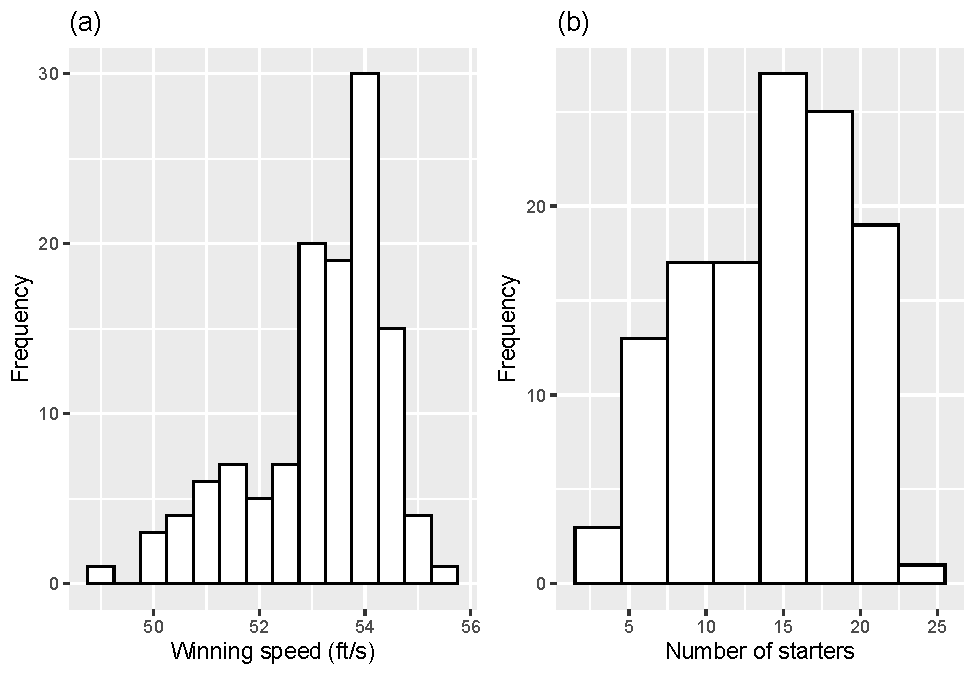
\includegraphics[width=0.9\linewidth]{bookdown-bysh_files/figure-latex/twohist-1} 

}

\caption{Histograms of key continuous variables.  Plot (a) shows winning speeds, while plot (b) shows the number of starters.}\label{fig:twohist}
\end{figure}

In Figure \ref{fig:twohist}(a), we see that the primary response, winning speed, follows a distribution with a slight left skew, with a large number of horses winning with speeds between 53-55 feet per second. Plot (b) shows that the number of starters is mainly distributed between 5 and 20, with the largest number of races having between 15 and 20 starters.

The primary categorical explanatory variable is track condition, where 88 (72\%) of the 122 races were run under fast conditions, 10 (8\%) under good conditions, and 24 (20\%) under slow conditions.

\hypertarget{bivariate-summaries}{%
\subsection{Bivariate Summaries}\label{bivariate-summaries}}

The next step in an initial exploratory analysis is the examination of numerical and graphical summaries of relationships between model covariates and responses. Figure \ref{fig:bivariate} is densely packed with illustrations of bivariate relationships. The relationship between two continuous variables is depicted with scatterplots below the diagonal and correlation coefficients above the diagonal. Here, we see that higher winning speeds are associated with more recent years, while the relationship between winning speed and number of starters is less clear cut. We also see a somewhat strong correlation between year and number of starters---we should be aware of highly correlated explanatory variables whose contributions might overlap too much.

\begin{figure}

{\centering 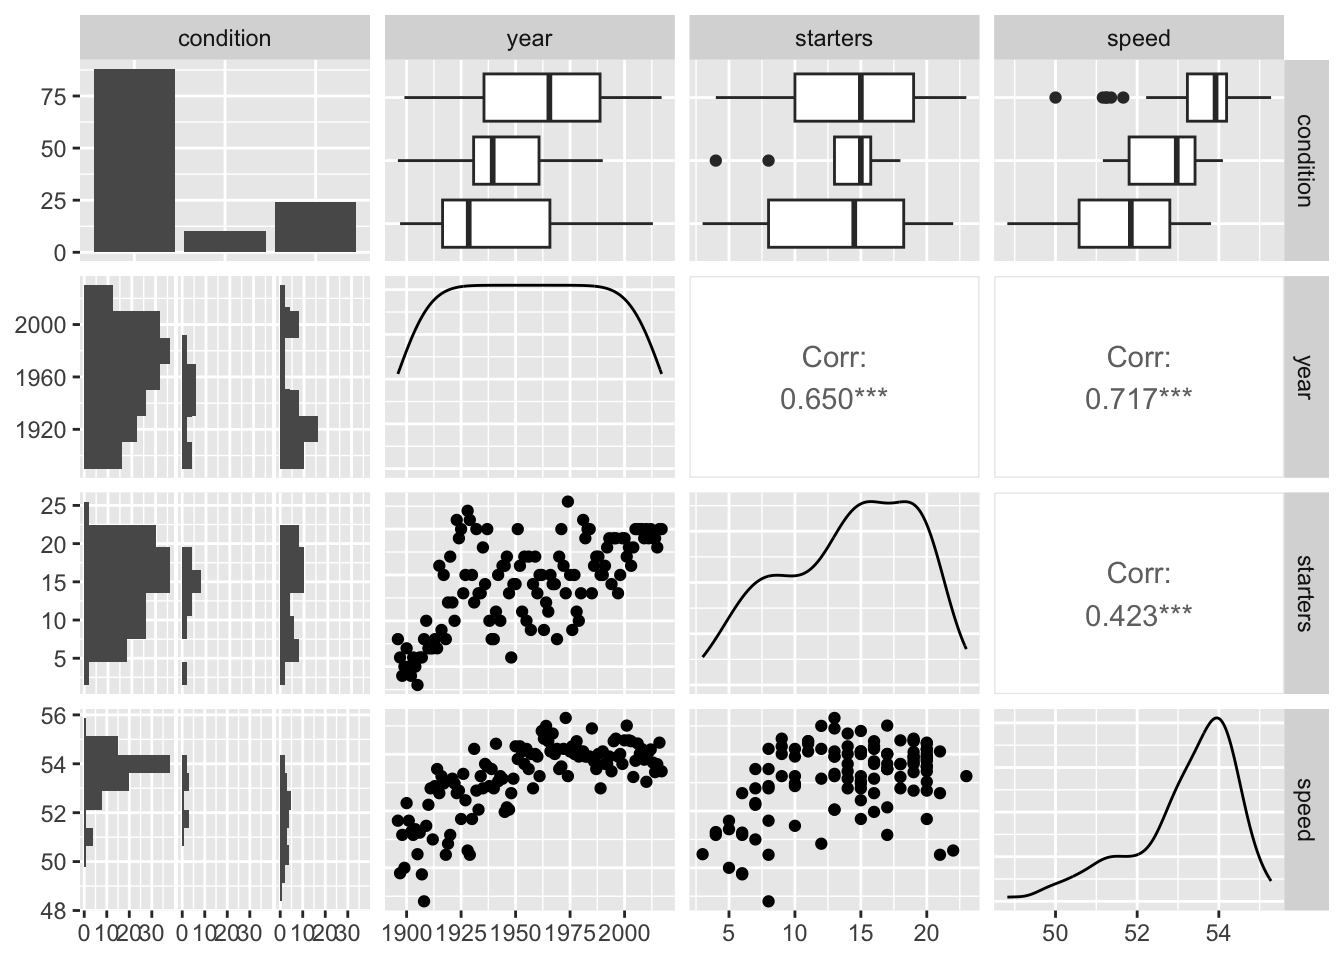
\includegraphics[width=0.9\linewidth]{bookdown-bysh_files/figure-latex/bivariate-1} 

}

\caption{Relationships between pairs of variables in the Kentucky Derby data set}\label{fig:bivariate}
\end{figure}

Relationships between categorical variables like track condition and continuous variables can be illustrated with side-by-side boxplots as in the top row, or with stacked histograms as in the first column. As expected, we see evidence of higher speeds on fast tracks and also a tendency for recent years to have more fast conditions. These observed trends can be supported with summary statistics generated by subgroup. For instance, the mean speed under fast conditions is 53.6 feet per second, compared to 52.7 ft/s under good conditions and 51.7 ft/s under slow conditions. Variability in winning speeds, however, is greatest under slow conditions (SD = 1.36 ft/s) and least under fast conditions (0.94 ft/s).

Finally, notice that the diagonal illustrates the distribution of individual variables, using density curves for continuous variables and a bar chart for categorical variables. Trends observed in the last two diagonal entries match trends observed in Figure \ref{fig:twohist}.

By using shape or color or other attributes, we can incorporate the effect of a third or even fourth variable into the scatterplots of Figure \ref{fig:bivariate}. For example, in the \textbf{coded scatterplot} of Figure \ref{fig:codeds} we see that speeds are generally faster under fast conditions, but the rate of increasing speed over time is greater under good or slow conditions.

\begin{figure}

{\centering 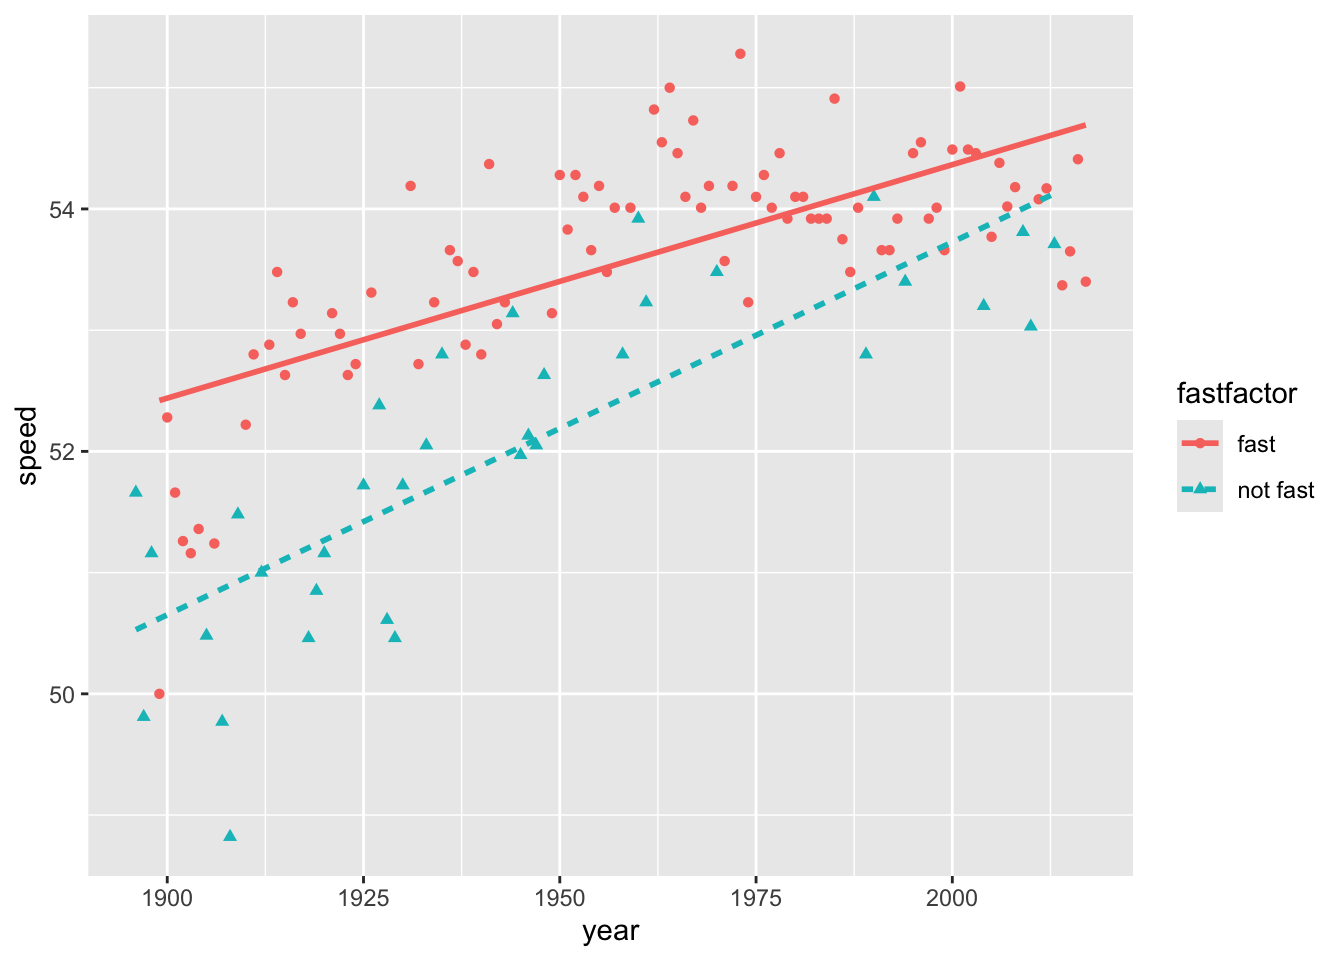
\includegraphics[width=0.9\linewidth]{bookdown-bysh_files/figure-latex/codeds-1} 

}

\caption{Linear trends in winning speeds over time, presented separately for fast conditions vs. good or slow conditions}\label{fig:codeds}
\end{figure}

Of course, any graphical analysis is exploratory, and any notable trends at this stage should be checked through formal modeling. At this point, a statistician begins to ask familiar questions such as:

\begin{itemize}
\tightlist
\item
  are winning speeds increasing in a linear fashion?
\item
  does the rate of increase in winning speed depend on track condition or number of starters?
\item
  after accounting for other explanatory variables, is greater field size (number of starters) associated with faster winning speeds (because more horses in the field means a greater chance one horse will run a very fast time) or slower winning speeds (because horses are more likely to bump into each other or crowd each others' attempts to run at full gait)?
\item
  are any of these associations statistically significant?
\item
  how well can we predict the winning speed in the Kentucky Derby?
\end{itemize}

As you might expect, answers to these questions will arise from proper consideration of variability and properly identified statistical models.

\hypertarget{multreg}{%
\section{Multiple linear regression modeling}\label{multreg}}

\hypertarget{SLRcontinuous}{%
\subsection{Simple linear regression with a continuous predictor}\label{SLRcontinuous}}

We will begin by modeling the winning speed as a function of time; for example, have winning speeds increased at a constant rate since 1896? For this initial model, let \(Y_{i}\) be the speed of the winning horse in year \(i\). Then, we might consider Model 1:

\begin{equation}
 Y_{i}=\beta_{0}+\beta_{1}(\textrm{Year}_{i})+\epsilon_{i} \quad \textrm{where} \quad \epsilon_{i}\sim \textrm{N}(0,\sigma^2).
\label{eq:model1}
\end{equation}

In this case, \(\beta_{0}\) represents the true intercept---the expected winning speed during Year 0. \(\beta_{1}\) represents the true slope---the expected increase in winning speed from one year to the next, assuming the rate of increase is linear (i.e., constant with each successive year since 1896). Finally, the \textbf{error} (\(\epsilon_{i}\)) terms represent the deviations of the actual winning speed in Year \(i\) (\(Y_i\)) from the expected scores under this model (\(\beta_{0}+\beta_{1}(\textrm{Year}_{i})\))---the part of a horse's winning speed that is not explained by a linear trend over time. The variability in these deviations from the regression model is denoted by \(\sigma^2\).

The parameters in this model (\(\beta_{0}\), \(\beta_{1}\), and \(\sigma^2\)) can be estimated through OLS methods; we will use hats to denote estimates of population parameters based on empirical data. Values for \(\hat{\beta}_{0}\) and \(\hat{\beta}_{1}\) are selected to minimize the sum of squared residuals, where a \textbf{residual} is simply the observed prediction error---the actual winning speed for a given year minus the winning speed predicted by the model. In the notation of this section,

\begin{itemize}
\tightlist
\item
  Predicted speed: \(\hat{Y}_{i}=\hat{\beta}_{0}+\hat{\beta}_{1}(\textrm{Year}_{i})\)
\item
  Residual (estimated error): \(\hat{\epsilon}_{i}=Y_{i} - \hat{Y}_{i}\)
\item
  Estimated variance of points around the line: \(\hat{\sigma}^2 = \sum \hat{\epsilon}^2_{i} / (n-2)\)
\end{itemize}

Using Kentucky Derby data, we estimate \(\hat{\beta}_{0}=2.05\), \(\hat{\beta}_{1}=0.026\), and \(\hat{\sigma}=0.90\). Thus, according to our simple linear regression model, winning horses of the Kentucky Derby have an estimated winning speed of 2.05 ft/s in Year 0 (more than 2000 years ago!), and the winning speed improves by an estimated 0.026 ft/s every year. With an \(R^2\) of 0.513, the regression model explains a moderate amount (51.3\%) of the year-to-year variability in winning speeds, and the trend toward a linear rate of improvement each year is statistically significant at the 0.05 level (t(120) = 11.251, p \textless{} .001).

\begin{verbatim}
lm(formula = speed ~ year, data = derby.df)

Coefficients:
            Estimate Std. Error t value Pr(>|t|)    
(Intercept) 2.053473   4.543754   0.452    0.652    
year        0.026126   0.002322  11.251   <2e-16 ***
---
Residual standard error: 0.9032 on 120 degrees of freedom
Multiple R-squared:  0.5134,    Adjusted R-squared:  0.5093 
\end{verbatim}

You may have noticed in Model 1 that the intercept has little meaning in context, since it estimates a winning speed in Year 0, when the first Kentucky Derby run at the current distance (1.25 miles) was in 1896. One way to create more meaningful parameters is through \textbf{centering}. In this case, we could create a centered year variable by subtracting 1896 from each year for Model 2:
\begin{equation}
\begin{split}
Y_{i}=\beta_{0}+\beta_{1}(\textrm{Yearnew}_{i})+\epsilon_{i}\quad &\textrm{where} \quad \epsilon_{i}\sim \textrm{N}(0,\sigma^2) \\
    &\textrm{and} \quad \textrm{Yearnew}=\textrm{Year}-1896.
\end{split}
\label{eq:model2}
\end{equation}
Note that the only thing that changes from Model 1 to Model 2 is the estimated intercept; \(\hat{\beta}_{1}\), \(R^2\), and \(\hat{\sigma}\) all remain exactly the same. Now \(\hat{\beta}_{0}\) tells us that the estimated winning speed in 1896 is 51.59 ft/s, but estimates of the linear rate of improvement or the variability explained by the model remain the same. As Figure \ref{fig:center} shows, centering year has the effect of shifting the y-axis from year 0 to year 1896, but nothing else changes.

\begin{verbatim}
lm(formula = speed ~ yearnew, data = derby.df)

Coefficients:
             Estimate Std. Error t value Pr(>|t|)    
(Intercept) 51.588393   0.162549  317.37   <2e-16 ***
yearnew      0.026126   0.002322   11.25   <2e-16 ***
---
Residual standard error: 0.9032 on 120 degrees of freedom
Multiple R-squared:  0.5134,    Adjusted R-squared:  0.5093 
\end{verbatim}

\begin{figure}

{\centering 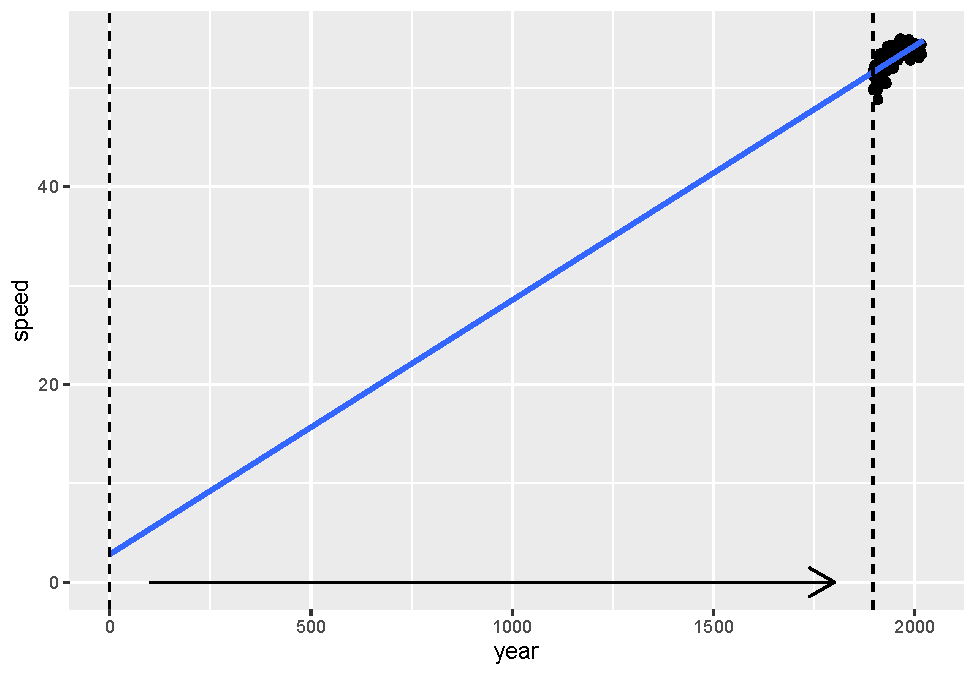
\includegraphics[width=0.9\linewidth]{bookdown-bysh_files/figure-latex/center-1} 

}

\caption{Compare Model 1 (with intercept at 0) to Model 2 (with intercept at 1896)}\label{fig:center}
\end{figure}

We should also attempt to verify that our LINE linear regression model assumptions fit for Model 2 if we want to make inferential statements (hypothesis tests or confidence intervals) about parameters or predictions. Most of these assumptions can be checked graphically using a set of residual plots as in Figure \ref{fig:resid2}:

\begin{itemize}
\tightlist
\item
  The upper left plot, Residuals vs.~Fitted, can be used to check the Linearity assumption. Residuals should be patternless around Y = 0; if not, there is a pattern in the data that is currently unaccounted for.
\item
  The upper right plot, Normal Q-Q, can be used to check the Normality assumption. Deviations from a straight line indicate that the distribution of residuals does not conform to a theoretical normal curve.
\item
  The lower left plot, Scale-Location, can be used to check the Equal Variance assumption. Positive or negative trends across the fitted values indicate variability that is not constant.
\item
  The lower right plot, Residuals vs.~Leverage, can be used to check for influential points. Points with high leverage (having unusual values of the predictors) and/or high absolute residuals can have an undue influence on estimates of model parameters.
\end{itemize}

\begin{figure}

{\centering 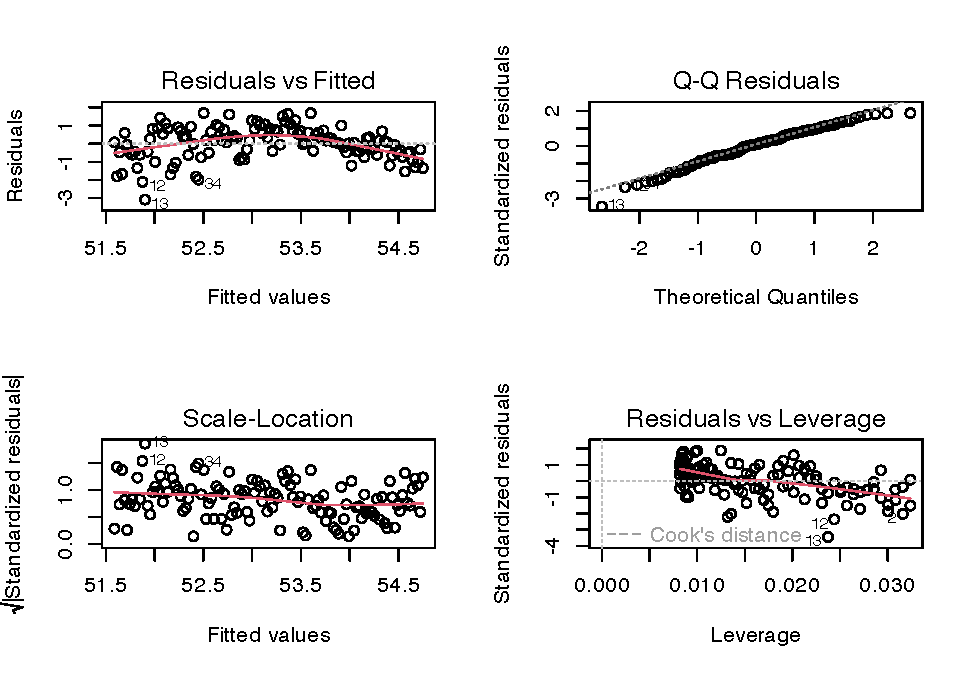
\includegraphics[width=0.9\linewidth]{bookdown-bysh_files/figure-latex/resid2-1} 

}

\caption{Residual plots for Model 2}\label{fig:resid2}
\end{figure}

In this case, the Residuals vs.~Fitted plot indicates that a quadratic fit might be better than the linear fit of Model 2; other assumptions look reasonable. Influential points would be denoted by high values of Cook's Distance; they would fall outside cutoff lines in the northeast or southeast section of the Residuals vs.~Leverage plot. Since no cutoff lines are even noticeable, there are no potential influential points of concern.

We recommend relying on graphical evidence for identifying regression model assumption violations, looking for highly obvious violations of assumptions before trying corrective actions. While some numerical tests have been devised for issues such as normality and influence, most of these tests are not very reliable, highly influenced by sample size and other factors. There is typically no residual plot, however, to evaluate the Independence assumption; evidence for lack of independence comes from knowing about the study design and methods of data collection. In this case, with a new field of horses each year, the assumption of independence is pretty reasonable.

Based on residual diagnostics, we should test Model 2Q, in which a quadratic term is added to the linear term in Model 2.\\
\begin{equation}
Y_{i}=\beta_{0}+\beta_{1}(\textrm{Yearnew}_{i})+\beta_{2}(\textrm{Yearnew}^2_{i})+\epsilon_{i}\quad \textrm{where}\quad \epsilon_{i}\sim \textrm{N}(0,\sigma^2).
\label{eq:model2Q}
\end{equation}
This model could suggest, for example, that the rate of increase in winning speeds is slowing down over time. In fact, there is evidence that the quadratic model improves upon the linear model (see Figure \ref{fig:models2and2q}). \(R^2\), the proportion of year-to-year variability in winning speeds explained by the model, has increased from 51.3\% to 64.1\%, and the pattern in the Residuals vs.~Fitted plot of Figure \ref{fig:resid2} has disappeared in Figure \ref{fig:resid2q}, although normality is a little sketchier in the left tail, and the larger mass of points with fitted values near 54 appears to have slightly lower variability. The significantly negative coefficient for \(\beta_{2}\) suggests that the rate of increase is indeed slowing in more recent years.

\begin{figure}

{\centering 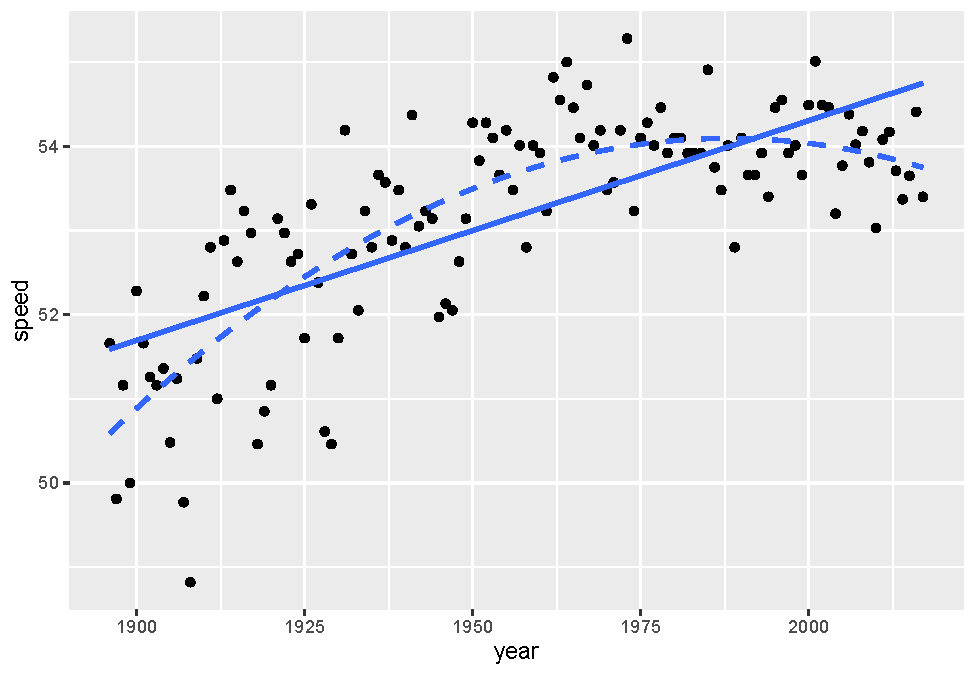
\includegraphics[width=0.9\linewidth]{bookdown-bysh_files/figure-latex/models2and2q-1} 

}

\caption{Linear vs. quadratic fit}\label{fig:models2and2q}
\end{figure}

\begin{verbatim}
lm(formula = speed ~ yearnew + yearnew2, data = derby.df)

Coefficients:
              Estimate Std. Error t value Pr(>|t|)    
(Intercept)  5.059e+01  2.082e-01 243.010  < 2e-16 ***
yearnew      7.617e-02  7.950e-03   9.581  < 2e-16 ***
yearnew2    -4.136e-04  6.359e-05  -6.505 1.92e-09 ***
---
Residual standard error: 0.779 on 119 degrees of freedom
Multiple R-squared:  0.641, Adjusted R-squared:  0.635 
\end{verbatim}

\begin{figure}

{\centering 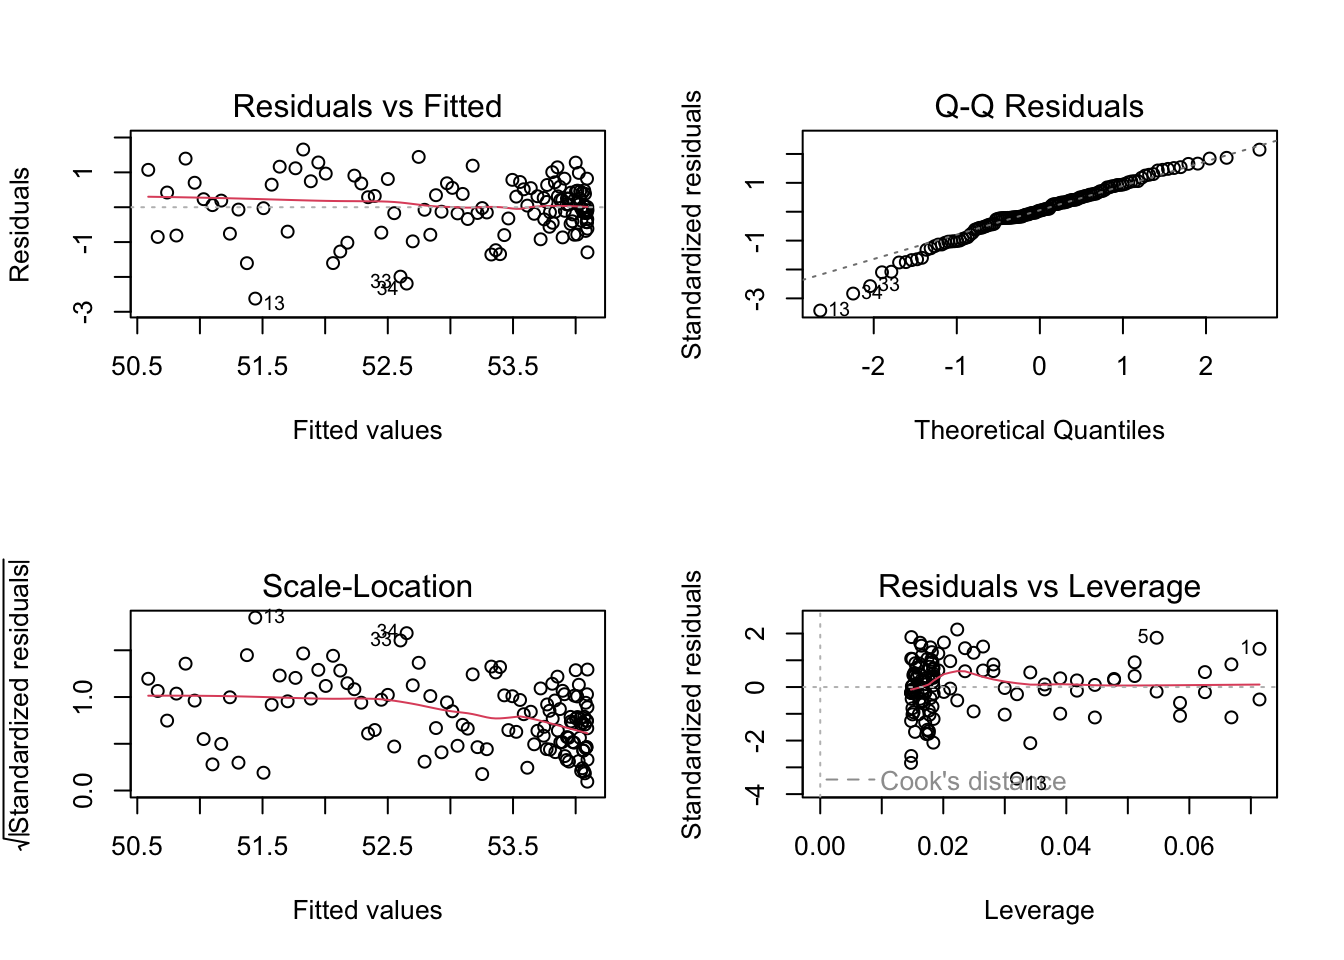
\includegraphics[width=0.9\linewidth]{bookdown-bysh_files/figure-latex/resid2q-1} 

}

\caption{Residual plots for Model 2Q}\label{fig:resid2q}
\end{figure}

\hypertarget{linear-regression-with-a-binary-predictor}{%
\subsection{linear regression with a binary predictor}\label{linear-regression-with-a-binary-predictor}}

We also may want to include track condition as an explanatory variable. We could start by using \texttt{fast} as the lone predictor: Do winning speeds differ for fast and non-fast conditions? \texttt{fast} is considered an \textbf{indicator variable}---it takes on only the values 0 and 1, where 1 indicates presence of a certain attribute (like fast racing conditions). Since \texttt{fast} is numeric, we can use simple linear regression techniques to fit Model 3:

\begin{equation}
Y_{i}=\beta_{0}+\beta_{1}(\textrm{Fast}_{i})+\epsilon_{i}\quad \textrm{where}\quad \epsilon_{i}\sim \textrm{N}(0,\sigma^2).
\label{eq:model3}
\end{equation}

Here, it's easy to see the meaning of our slope and intercept by writing out separate equations for the two conditions:

\begin{itemize}
\tightlist
\item
  Good or slow conditions (\texttt{fast} = 0)
\end{itemize}

\begin{equation}
Y_{i} = \beta_{0}+\epsilon_{i}
\end{equation}

\begin{itemize}
\tightlist
\item
  Fast conditions (\texttt{fast} = 1)
\end{itemize}

\begin{equation}
Y_{i} = (\beta_{0}+\beta_{1})+\epsilon_{i}
\end{equation}

\(\beta_{0}\) is the expected winning speed under good or slow conditions, while \(\beta_{1}\) is the difference between expected winning speeds under fast conditions vs.~non-fast conditions. According to our fitted Model 3, the estimated winning speed under non-fast conditions is 52.0 ft/s, while mean winning speeds under fast conditions are estimated to be 1.6 ft/s higher.

\begin{verbatim}
lm(formula = speed ~ fast, data = derby.df)

Coefficients:
            Estimate Std. Error t value Pr(>|t|)    
(Intercept)  51.9938     0.1826 284.698  < 2e-16 ***
fast          1.6292     0.2150   7.577 8.17e-12 ***
---
Residual standard error: 1.065 on 120 degrees of freedom
Multiple R-squared:  0.3236,    Adjusted R-squared:  0.318 
\end{verbatim}

You might be asking at this point: If we simply wanted to compare mean winning speeds under fast and non-fast conditions, why didn't we just run a two-sample t-test? The answer is: we did! The t-test corresponding to \(\beta_{1}\) is equivalent to an independent-samples t-test with under equal variances. Convince yourself that this is true, and that the equal variance assumption is needed.

\hypertarget{multiple-linear-regression-with-two-predictors}{%
\subsection{Multiple linear regression with two predictors}\label{multiple-linear-regression-with-two-predictors}}

The beauty of the linear regression framework is that we can add additional explanatory variables in order to explain more variability in our response, obtain better and more precise predictions, and control for certain covariates while evaluating the effect of others. For example, we could consider adding \texttt{yearnew} to Model 3, which has the indicator variable \texttt{fast} as its only predictor. In this way, we would estimate the difference between winning speeds under fast and non-fast conditions \emph{after accounting for the effect of time}. As we observed in Figure \ref{fig:bivariate}, recent years have tended to have more races under fast conditions, so Model 3 might overstate the effect of fast conditions because winning speeds have also increased over time. A model with terms for both year and track condition will estimate the difference between winning speeds under fast and non-fast conditions \emph{for a fixed year}; for example, if it had rained in 2016 and turned the track muddy, how much would we have expected the winning speed to decrease?

Our new model (Model 4) can be written:

\begin{equation}
Y_{i}=\beta_{0}+\beta_{1}(\textrm{Yearnew}_{i})+\beta_{2}(\textrm{Fast}_{i})+\epsilon_{i}\quad \textrm{where}\quad \epsilon_{i}\sim \textrm{N}(0,\sigma^2).
\label{eq:model4}
\end{equation}

and OLS provides the following parameter estimates:

\begin{verbatim}
lm(formula = speed ~ yearnew + fast, data = derby.df)

Coefficients:
             Estimate Std. Error t value Pr(>|t|)    
(Intercept) 50.917822   0.154602  329.35  < 2e-16 ***
yearnew      0.022583   0.001919   11.77  < 2e-16 ***
fast         1.226846   0.150721    8.14 4.39e-13 ***
---
Residual standard error: 0.7269 on 119 degrees of freedom
Multiple R-squared:  0.6874,    Adjusted R-squared:  0.6822 
\end{verbatim}

Our new model estimates that winning speeds are, on average, 1.23 ft/s faster under fast conditions after accounting for time trends, which is down from an estimated 1.63 ft/s without accounting for time. It appears our original model (Model 3) may have overestimated the effect of fast conditions by conflating it with improvements over time. Through our new model, we also estimate that winning speeds increase by 0.023 ft/s per year, after accounting for track condition. This yearly effect is also smaller than the 0.026 ft/s per year we estimated in Model 1, without adjusting for track condition. Based on the \(R^2\) value, Model 4 explains 68.7\% of the year-to-year variability in winning speeds, a noticeable increase over using either explanatory variable alone.

\hypertarget{multreg-inference}{%
\subsection{Inference in multiple linear regression: normal theory}\label{multreg-inference}}

So far we have been using linear regression for descriptive purposes, which is an important task. We are often interested in issues of statistical inference as well---determining if effects are statistically significant, quantifying uncertainty in effect size estimates with confidence intervals, and quantifying uncertainty in model predictions with prediction intervals. Under LINE assumptions, all of these inferential tasks can be completed with the help of the t-distribution and estimated standard errors.

Here are examples of inferential statements based on Model 4:

\begin{itemize}
\tightlist
\item
  We can be 95\% confident that average winning speeds under fast conditions are between 0.93 and 1.53 ft/s higher than under non-fast conditions, after accounting for the effect of year.
\item
  Fast conditions lead to significantly faster winning speeds than non-fast conditions (t = 8.14 on 119 df, p \textless{} .001), holding year constant.
\item
  Based on our model, we can be 95\% confident that the winning speed in 2017 under fast conditions will be between 53.4 and 56.3 ft/s. Note that Always Dreaming's actual winning speed barely fit within this interval---the 2017 winning speed was a borderline outlier on the slow side.
\end{itemize}

\begin{Shaded}
\begin{Highlighting}[]
\KeywordTok{confint}\NormalTok{(model4)}
\end{Highlighting}
\end{Shaded}

\begin{verbatim}
                  2.5 %      97.5 %
(Intercept) 50.61169473 51.22394836
yearnew      0.01878324  0.02638227
fast         0.92840273  1.52528902
\end{verbatim}

\begin{Shaded}
\begin{Highlighting}[]
\NormalTok{new.data <-}\StringTok{ }\KeywordTok{data.frame}\NormalTok{(}\DataTypeTok{yearnew =} \DecValTok{2017} \OperatorTok{-}\StringTok{ }\DecValTok{1896}\NormalTok{, }\DataTypeTok{fast =} \DecValTok{1}\NormalTok{) }
\KeywordTok{predict}\NormalTok{(model4, }\DataTypeTok{new =}\NormalTok{ new.data, }\DataTypeTok{interval =} \StringTok{"prediction"}\NormalTok{)}
\end{Highlighting}
\end{Shaded}

\begin{verbatim}
       fit     lwr      upr
1 54.87718 53.4143 56.34006
\end{verbatim}

\hypertarget{multreg-boot}{%
\subsection{Inference in multiple linear regression: bootstrapping}\label{multreg-boot}}

Remember that you must check LINE assumptions using the same residual plots as in Figure \ref{fig:resid2} to ensure that the inferential statements in the previous section are valid. In cases when model assumptions are shaky, one alternative approach to statistical inference is \textbf{bootstrapping}; in fact, bootstrapping is a robust approach to statistical inference that we will use frequently throughout this book because of its power and flexibility. In bootstrapping, we use only the data we've collected and computing power to estimate the uncertainty surrounding our parameter estimates. Our primary assumption is that our original sample represents the larger population, and then we can learn about uncertainty in our parameter estimates through repeated samples (with replacement) from our original sample.

If we wish to use bootstrapping to obtain confidence intervals for our coefficients in Model 4, we could follow these steps:

\begin{itemize}
\tightlist
\item
  take a (bootstrap) sample of 122 years of Derby data with replacement, so that some years will get sampled several times and others not at all. This is \textbf{case resampling}, so that all information from a given year (winning speed, track condition, number of starters) remains together.
\item
  fit Model 4 to the bootstrap sample, saving \(\hat{\beta}_0\), \(\hat{\beta}_1\), and \(\hat{\beta}_2\).
\item
  repeat the two steps above a large number of times (say 1000)
\item
  the 1000 bootstrap estimates for each parameter can be plotted to show the \textbf{bootstrap distribution} (see Figure \ref{fig:boot4})
\item
  a 95\% confidence interval for each parameter can be found by taking the middle 95\% of each bootstrap distribution---i.e., by picking off the 2.5 and 97.5 percentiles. This is called the \textbf{percentile method}.
\end{itemize}

\begin{Shaded}
\begin{Highlighting}[]
    \CommentTok{# updated code from tobiasgerstenberg on github}
    \KeywordTok{library}\NormalTok{(rsample)}
    \KeywordTok{library}\NormalTok{(purrr)}
    \KeywordTok{library}\NormalTok{(broom)}
\NormalTok{    bootreg =}\StringTok{ }\NormalTok{derby.df }\OperatorTok\StringTok{ }
\StringTok{      }\KeywordTok{bootstraps}\NormalTok{(}\DecValTok{1000}\NormalTok{) }\OperatorTok
\StringTok{      }\KeywordTok{pull}\NormalTok{(splits) }\OperatorTok\StringTok{ }
\StringTok{      }\KeywordTok{map_dfr}\NormalTok{(}\OperatorTok{~}\KeywordTok{lm}\NormalTok{(speed }\OperatorTok{~}\StringTok{ }\NormalTok{yearnew }\OperatorTok{+}\StringTok{ }\NormalTok{fast, }\DataTypeTok{data =}\NormalTok{ .) }\OperatorTok\StringTok{ }
\StringTok{                }\KeywordTok{tidy}\NormalTok{())}
\NormalTok{    summarize =}\StringTok{ }\NormalTok{dplyr}\OperatorTok{::}\NormalTok{summarize}
\NormalTok{    bootreg }\OperatorTok\StringTok{ }
\StringTok{      }\KeywordTok{group_by}\NormalTok{(term) }\OperatorTok\StringTok{ }
\StringTok{      }\KeywordTok{summarize}\NormalTok{(}\DataTypeTok{low=}\KeywordTok{quantile}\NormalTok{(estimate, }\FloatTok{.025}\NormalTok{),}
            \DataTypeTok{high=}\KeywordTok{quantile}\NormalTok{(estimate, }\FloatTok{.975}\NormalTok{))}
\end{Highlighting}
\end{Shaded}

\begin{verbatim}
# A tibble: 3 x 3
  term            low    high
  <chr>         <dbl>   <dbl>
1 (Intercept) 50.6    51.3   
2 fast         0.929   1.56  
3 yearnew      0.0183  0.0268
\end{verbatim}

\begin{figure}

{\centering 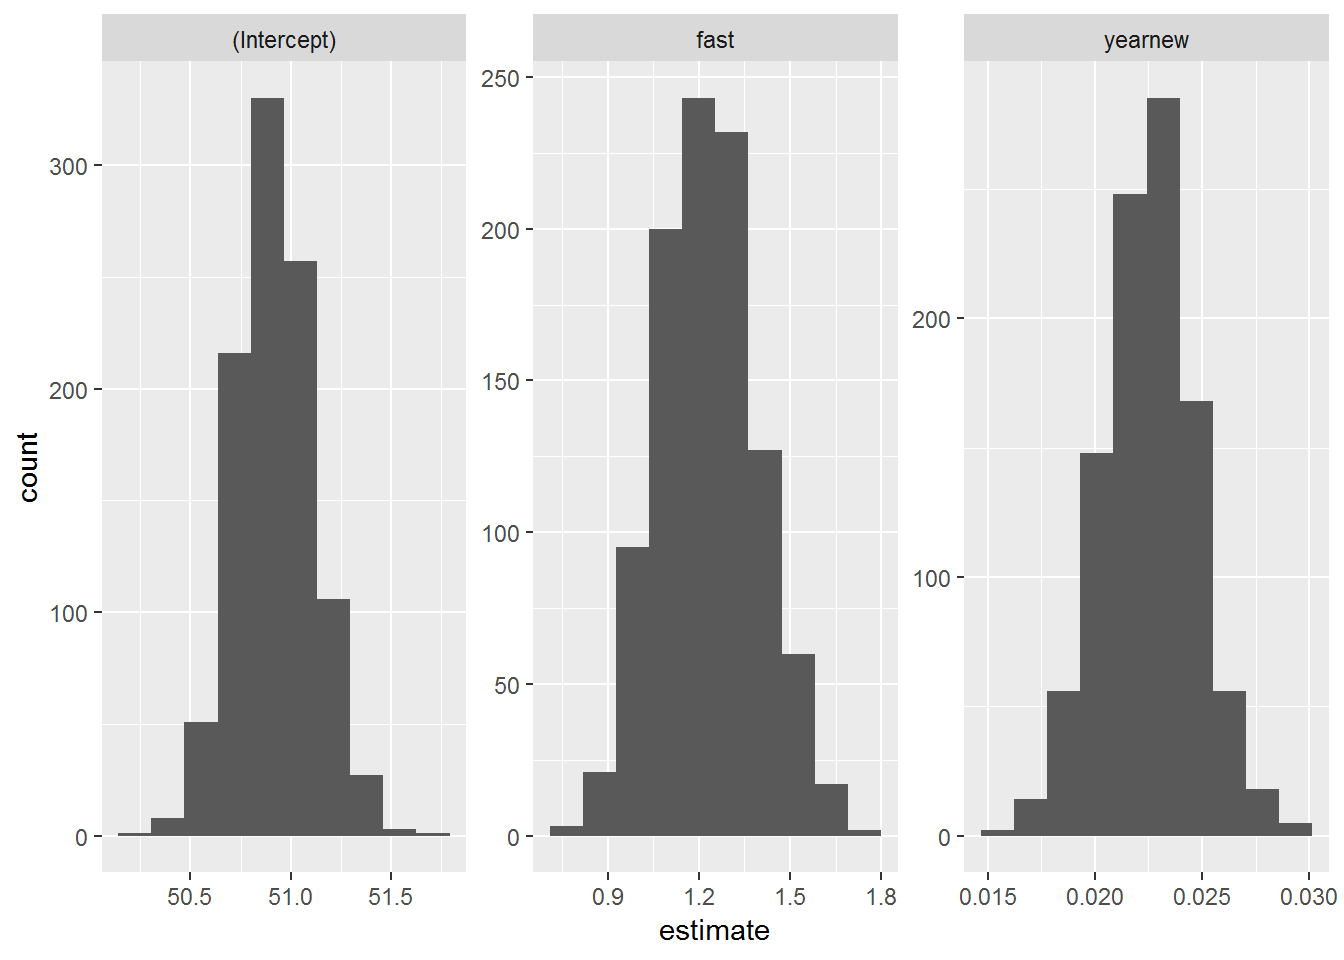
\includegraphics[width=0.9\linewidth]{bookdown-bysh_files/figure-latex/boot4-1} 

}

\caption{Bootstrapped distributions for Model 4 coefficients}\label{fig:boot4}
\end{figure}

In this case, we see that 95\% bootstrap confidence intervals for \(\beta_0\), \(\beta_1\), and \(\beta_2\) are very similar to the normal-theory confidence intervals we found earlier. For example, the normal-theory confidence interval for the effect of fast tracks is 0.93 to 1.53 ft/s, while the analogous bootstrap confidence interval is 0.89 to 1.55 ft/s.

There are many variations on this bootstrap procedure. For example, you could sample residuals rather than cases, or you could conduct a parametric bootstrap in which error terms are randomly chosen from a normal distribution. In addition, researchers have devised other ways of calculating confidence intervals besides the percentile method, including normality, studentized, and bias-corrected and accelerated (\citet{Hesterberg2015}; \citet{Efron1993}; \citet{Davison1997}). We will focus on case resampling and percentile confidence intervals for now for their understandability and wide applicability.

\hypertarget{multiple-linear-regression-with-an-interaction-term}{%
\subsection{Multiple linear regression with an interaction term}\label{multiple-linear-regression-with-an-interaction-term}}

Adding terms to form a multiple linear regression model as we did in Model 4 is a very powerful modeling tool, allowing us to account for multiple sources of uncertainty and to obtain more precise estimates of effect sizes after accounting for the effect of important covariates. One limitation of Model 4, however, is that we must assume that the effect of track condition has been the same for 122 years, or conversely that the yearly improvements in winning speeds are identical for all track conditions. To expand our modeling capabilities to allow the effect of one predictor to change depending on levels of a second predictor, we need to consider \textbf{interaction terms}. Amazingly, if we create a new variable by taking the product of \texttt{yearnew} and \texttt{fast} (i.e., the \textbf{interaction} between \texttt{yearnew} and \texttt{fast}), adding that variable into our model will have the desired effect.

Thus, consider Model 5:

\begin{equation}
\begin{split}
 Y_{i}&= \beta_{0}+\beta_{1}(\textrm{Yearnew}_{i})+\beta_{2}(\textrm{Fast}_{i}) \notag \\
      &{}+\beta_{3}(\textrm{Yearnew}\times\textrm{Fast}_{i})+\epsilon_{i}\quad \textrm{where}\quad \epsilon_{i}\sim \textrm{N}(0,\sigma^2).
\end{split}
\label{eq:model5}
\end{equation}

where OLS provides the following parameter estimates:

\begin{verbatim}
lm(formula = speed ~ yearnew + fast + yearnew:fast, data = derby.df)

Coefficients:
              Estimate Std. Error t value Pr(>|t|)    
(Intercept)  50.528629   0.205072 246.394  < 2e-16 ***
yearnew       0.030751   0.003471   8.859 9.84e-15 ***
fast          1.833523   0.262175   6.994 1.73e-10 ***
yearnew:fast -0.011490   0.004117  -2.791  0.00613 ** 
---
Residual standard error: 0.7071 on 118 degrees of freedom
Multiple R-squared:  0.7068,    Adjusted R-squared:  0.6993 
\end{verbatim}

According to OLS estimates, estimated winning speeds can be found by:

\begin{equation}
 \hat{Y}_{i}=50.53+0.031(\textrm{Yearnew}_{i})+1.83(\textrm{Fast}_{i})-0.011(\textrm{Yearnew}\times\textrm{Fast}_{i}).
\label{eq:model5est}
\end{equation}

Interpretations of model coefficients are most easily seen by writing out separate equations for fast and non-fast track conditions:

\begin{align*}
 \textrm{Fast}=0: & \\
 \hat{Y}_{i} &= 50.53+0.031(\textrm{Yearnew}_{i}) \\
 \textrm{Fast}=1: & \\
 \hat{Y}_{i} &= (50.53+1.83)+(0.031-0.011)(\textrm{Yearnew}_{i})
 \end{align*}

leading to the following interpretations for estimated model coefficients:

\begin{itemize}
\tightlist
\item
  \(\hat{\beta}_{0} = 50.53\). The expected winning speed in 1896 under non-fast conditions was 50.53 ft/s.
\item
  \(\hat{\beta}_{1} = 0.031\). The expected yearly increase in winning speeds under non-fast conditions is 0.031 ft/s.
\item
  \(\hat{\beta}_{2} = 1.83\). The winning speed in 1896 was expected to be 1.83 ft/s faster under fast conditions compared to non-fast conditions.
\item
  \(\hat{\beta}_{3} = -0.011\). The expected yearly increase in winning speeds under fast conditions is 0.020 ft/s, which is 0.011 ft/s less than the expected annual increase under non-fast conditions.
\end{itemize}

In fact, using interaction allows us to model the relationships we noticed in Figure \ref{fig:codeds}, where both the intercept and slope describing the relationships between \texttt{speed} and \texttt{year} differ depending on whether track conditions were fast or not. Note that we interpret the coefficient for the interaction term by comparing slopes under fast and non-fast conditions; this produces a much more understandable interpretation for a reader than attempting to interpret the -0.011 directly.

\hypertarget{multreg_build}{%
\subsection{Building a multiple linear regression model}\label{multreg_build}}

We now begin iterating toward a ``final model'' for these data, on which we will base conclusions. Typical features of a ``final multiple linear regression model'' include:

\begin{itemize}
\tightlist
\item
  explanatory variables allow one to address primary research questions
\item
  explanatory variables control for important covariates
\item
  potential interactions have been investigated
\item
  variables are centered where interpretations can be enhanced
\item
  unnecessary terms have been removed
\item
  LINE assumptions and the presence of influential points have both been checked using residual plots
\item
  the model tells a ``persuasive story parsimoniously''
\end{itemize}

Although the process of reporting and writing up research results often demands the selection of a sensible final model, it's important to realize that (a) statisticians typically will examine and consider an entire taxonomy of models when formulating conclusions, and (b) different statisticians sometimes select different models as their ``final model'' for the same set of data. Choice of a ``final model'' depends on many factors, such as primary research questions, purpose of modeling, tradeoff between parsimony and quality of fitted model, underlying assumptions, etc. Modeling decisions should never be automated or made completely on the basis of statistical tests; subject area knowledge should always play a role in the modeling process. You should be able to defend any final model you select, but you should not feel pressured to find the one and only ``correct model'', although most good models will lead to similar conclusions.

Several tests and measures of model performance can be used when comparing different models for model building:

\begin{itemize}
\tightlist
\item
  \(R^2\) we have seen; it measures the variability in the response variable explained by the model. One problem is that \(R^2\) always increases with extra predictors, even if the predictors add very little information.
\item
  adjusted \(R^2\). Adds a penalty for model complexity to \(R^2\) so that any increase in performance must outweigh the cost of additional complexity. We should ideally favor any model with higher adjusted \(R^2\), regardless of size, but the penalty for model complexity (additional terms) is fairly ad-hoc.
\item
  AIC (Akaike Information Criterion). Again attempts to balance model performance with model complexity, with smaller AIC levels being preferable, regardless of model size. The BIC (Bayesian Information Criterion) is similar to the AIC, but with a greater penalty for additional model terms.
\item
  extra sum of squares F test. This is a generalization of the t-test for individual model coefficients which can be used to perform significance tests on \textbf{nested models}, where one model is a reduced version of the other. For example, we could test whether our final model (below) really needs to adjust for track condition, which is comprised of indicators for both fast condition and good condition (leaving slow condition as the reference level). Our null hypothesis is then \(\beta_{3}=\beta_{4}=0\). We have statistically significant evidence (F = 57.2 on 2 and 116 df, p \textless{} .001) that track condition is associated with winning speeds, after accounting for quadratic time trends and number of starters.
\end{itemize}

One potential final model for predicting winning speeds of Kentucky Derby races is:

\begin{equation}
\begin{split}
 Y_{i}&=\beta_{0}+\beta_{1}(\textrm{Yearnew}_{i})+\beta_{2}(\textrm{Yearnew}^2_{i})+\beta_{3}(\textrm{Fast}_{i})\\
      &{}+\beta_{4}(\textrm{Good}_{i})+\beta_{5}(\textrm{Starters}_{i})+\epsilon_{i}\quad 
      \textrm{where}\quad \epsilon_{i}\sim \textrm{N}(0,\sigma^2).
\end{split}
\label{eq:model0}
\end{equation}

and OLS provides the following parameter estimates:

\begin{verbatim}
lm(formula = speed ~ yearnew + yearnew2 + fast + good + starters, 
    data = derby.df)

Coefficients:
              Estimate Std. Error t value Pr(>|t|)    
(Intercept)  5.002e+01  1.946e-01 256.980  < 2e-16 ***
yearnew      7.003e-02  6.130e-03  11.424  < 2e-16 ***
yearnew2    -3.697e-04  4.598e-05  -8.041 8.44e-13 ***
fast         1.393e+00  1.305e-01  10.670  < 2e-16 ***
good         9.157e-01  2.077e-01   4.409 2.33e-05 ***
starters    -2.528e-02  1.360e-02  -1.859   0.0656 .  
---
Residual standard error: 0.5483 on 116 degrees of freedom
Multiple R-squared:  0.8267,    Adjusted R-squared:  0.8192 
\end{verbatim}

\begin{verbatim}
Analysis of Variance Table

Model 1: speed ~ yearnew + yearnew2 + starters
Model 2: speed ~ yearnew + yearnew2 + fast + good + starters
  Res.Df    RSS Df Sum of Sq      F    Pr(>F)    
1    118 69.257                                  
2    116 34.870  2    34.386 57.196 < 2.2e-16 ***
\end{verbatim}

This model accounts for the slowing annual increases in winning speed with a negative quadratic term, adjusts for baseline differences stemming from track conditions, and suggests that, for a fixed year and track condition, a larger field is associated with slower winning times (unlike the positive relationship we saw between speed and number of starters in our exploratory analyses). The model explains 82.7\% of the year-to-year variability in winning speeds, and residual plots show no serious issues with LINE assumptions. We tested interaction terms for different effects of time or number of starters based on track condition, but we found no significant evidence of interactions.

\hypertarget{preview}{%
\section{Preview}\label{preview}}

Having reviewed key ideas from multiple linear regression, you are now ready to extend those ideas, especially to handle non-normal responses and lack of independence. This section provides a preview of the type of problems you will encounter in the book. For each journal article cited, we provide an abstract in the authors' words, a description of the type of response and, when applicable, the structure of the data. Each of these examples appears later as an exercise, where you can play with the actual data or evaluate the analyses detailed in the articles.

\hypertarget{soccer}{%
\subsection{Soccer}\label{soccer}}

\citet{Roskes2011} . The right side? Under time pressure, approach motivation leads to right-oriented bias. \emph{Psychological Science} {[}Online{]} \textbf{22(11)}:1403-7. DOI: 10.1177/0956797611418677, October 2011.

\begin{quote}
\textbf{Abstract:} Approach motivation, a focus on achieving positive outcomes, is related to relative left-hemispheric brain activation, which translates to a variety of right-oriented behavioral biases. \([\ldots]\) In our analysis of all Federation Internationale de Football Association (FIFA) World Cup penalty shoot-outs, we found that goalkeepers were two times more likely to dive to the right than to the left when their team was behind, a situation that we conjecture induces approach motivation. Because penalty takers shot toward the two sides of the goal equally often, the goalkeepers' right-oriented bias was dysfunctional, allowing more goals to be scored.
\end{quote}

The response for this analysis is the direction of the goalkeeper dive, a binary variable. For example, you could let Y=1 if the dive is to the right and Y=0 if the dive is to the left. This response is clearly not normally distributed. One approach to the analysis is logistic regression as described in Chapter \ref{ch-logreg}. A binomial random variable could also be created for this application by summing the binary variables for each game so that Y= the number of dives right out of the number of dives the goalkeeper makes during a game. {[}Thought question: Do you buy the last line of the abstract?{]}

\hypertarget{elephant-mating}{%
\subsection{Elephant Mating}\label{elephant-mating}}

\citet{Poole1989} . Mate guarding, reproductive success and female choice in African elephants. \emph{Animal Behavior} \textbf{37}:842-49.

\begin{quote}
\textbf{Abstract:} Male guarding of females, male mating success and female choice were studied for 8 years among a population of African elephants, Loxodonta africana. Males were not able to compete successfully for access to oestrous female until approximately 25 years of age. Males between 25 and 35 years of age obtained matings during early and late oestrus, but rarely in mid-oestrus. Large musth males over 35 years old guarded females in mid-oestrus. Larger, older males ranked above younger, smaller males and the number of females guarded by males increased rapidly late in life. Body size and longevity are considered important factors in determining the lifetime reproductive success of male elephants\ldots{}
\end{quote}

Poole and her colleagues recorded, for each male elephant, his age (in years) and the number of matings for a given year. The researchers were interested in how age affects the males' mating patterns. Specifically, questions concern whether there is a steady increase in mating success as an elephant ages or if there is an optimal age after which the number of matings decline. Because the responses of interest are counts (number of matings for each elephant for a given year), we will consider a Poisson regression (see Chapter \ref{ch-poissonreg}). The general form for Poisson responses is the number of events for a specified time, volume, or space.

\hypertarget{parenting-and-gang-activity}{%
\subsection{Parenting and Gang Activity}\label{parenting-and-gang-activity}}

\citet{Walker-Barnes2001} . Ethnic differences in the effect of parenting on gang involvement and gang delinquency: a longitudinal, hierarchical linear modeling perspective. \emph{Child Development} \textbf{72(6)}:1814-31.

\begin{quote}
\textbf{Abstract:} This study examined the relative influence of peer and parenting behavior on changes in adolescent gang involvement and gang-related delinquency. An ethnically diverse sample of 300 ninth-grade students was recruited and assessed on eight occasions during the school year. Analyses were conducted using hierarchical linear modeling. Results indicated that, in general, adolescents decreased their level of gang involvement over the course of the school year, whereas the average level of gang delinquency remained constant over time. As predicted, adolescent gang involvement and gang-related delinquency were most strongly predicted by peer gang involvement and peer gang delinquency, respectively. Nevertheless, parenting behavior continued to significantly predict change in both gang involvement and gang delinquency, even after controlling for peer behavior. A significant interaction between parenting and ethnic and cultural heritage found the effect of parenting to be particularly salient for Black students, for whom higher levels of behavioral control and lower levels of lax parental control were related to better behavioral outcomes over time, whereas higher levels of psychological control predicted worse behavioral outcomes.
\end{quote}

The response for this study is a gang activity measure which ranges from 1 to 100. While it may be reasonable to assume this measure is approximately normal, the structure of this data implies that it is not a simple regression problem. Individual students have measurements made at 8 different points in time. We cannot assume that we have 2400 independent observations because the same measurements on one individual are more likely to be similar than a measurement of another student. Multilevel modeling as discussed in Chapter \ref{ch-lon} can often be used in these situations.

\hypertarget{crime}{%
\subsection{Crime}\label{crime}}

\citet{Gelman2007} . An analysis of the NYPD's stop-and-frisk policy in the context of claims of racial bias. \emph{Journal of the American Statistical Association} \textbf{102(479)}:813-823.

\begin{quote}
\textbf{Abstract:} Recent studies by police departments and researchers confirm that police stop racial and ethnic minority citizens more often than whites, relative to their proportions in the population. However, it has been argued stop rates more accurately reflect rates of crimes committed by each ethnic group, or that stop rates reflect elevated rates in specific social areas such as neighborhoods or precincts. Most of the research on stop rates and police-citizen interactions has focused on traffic stops, and analyses of pedestrian stops are rare. In this paper, we analyze data from 175,000 pedestrian stops by the New York Police Department over a fifteen-month period. We disaggregate stops by police precinct, and compare stop rates by racial and ethnic group controlling for previous race-specific arrest rates. We use hierarchical multilevel models to adjust for precinct-level variability, thus directly addressing the question of geographic heterogeneity that arises in the analysis of pedestrian stops. We find that persons of African and Hispanic descent were stopped more frequently than whites, even after controlling for precinct variability and race-specific estimates of crime participation.
\end{quote}

This application involves both non-normal data (number of stops by ethnic group can be modeled as a Poisson response) and multilevel data (number of stops within precincts will likely be correlated due to characteristics of the precinct population). This type of analysis will be the last type you encounter, generalized linear multilevel modeling, as addressed in Chapter \ref{ch-GLMM}.

\hypertarget{exercises}{%
\section{Exercises}\label{exercises}}

\hypertarget{conceptual-exercises}{%
\subsection{Conceptual Exercises}\label{conceptual-exercises}}

\begin{enumerate}
\def\labelenumi{\arabic{enumi}.}
\item
  \textbf{Applications that do not violate the OLS assumptions for inference}. Identify the response and explanatory variable(s) for each problem. Write the OLS assumptions for inference in the context of each study.

  \begin{enumerate}
  \def\labelenumii{\alph{enumii}.}
  \tightlist
  \item
    \textbf{Cricket Chirps.} Researchers record the number of cricket chirps per minute and temperature during that time to investigate whether the number of chirps varies with the temperature.
  \item
    \textbf{Women's Heights.} A random selection of women aged 20-24 years are selected and their shoe size is used to predict their height\\
  \end{enumerate}
\item
  \textbf{Applications that do violate the OLS assumptions for inference}. All of the examples in this section have at least one violation of the OLS assumptions for inference. Begin by identifying the response and explanatory variables. Then, identify which OLS assumption(s) are violated.

  \begin{enumerate}
  \def\labelenumii{\alph{enumii}.}
  \tightlist
  \item
    \textbf{Low Birthweights.} Researchers are attempting to see if socioeconomic status and parental stability are predictive of low birthweight. They classify a child as having a low birthweight if their birthweight is less than 2,500 grams.
  \item
    \textbf{Clinical Trial I.} A Phase II clinical trial is designed to compare the number of patients getting relief at different dose levels. 100 patients get dose A, 100 get dose B, and 100 get dose C.
  \item
    \textbf{Canoes and zip codes.} For each of over 27,000 overnight permits for the Boundary Water Canoe area, the zip code for the group leader has been translated to the distance traveled and socioeconomic data. This data is used to create a model for the number of trips made per zip code.
  \item
    \textbf{Clinical Trial II.} A randomized clinical trial investigated postnatal depression and the use of an estrogen patch. Patients were randomly assigned to either use the patch or not. Depression scores were recorded on 6 different visits.
  \item
    \textbf{Elephant mating.} Researchers are interested in how elephant age affects mating patterns among males. In particular, do older elephants have greater mating success, and is there an optimal age for mating among males? Data collected includes, for each elephant, age and number of matings in a given year.\\
  \end{enumerate}
\item
  \textbf{Kentucky Derby.} The next set of questions is related to the Kentucky Derby case study from this chapter.

  \begin{enumerate}
  \def\labelenumii{\alph{enumii}.}
  \tightlist
  \item
    Discuss the pros and cons of using side-by-side boxplots vs.~stacked histograms to illustrate the relationships between year and track condition in Figure \ref{fig:bivariate}.
  \item
    Why is a scatterplot more informative than a correlation coefficient to describe the relationship between speed of the winning horse and year in Figure \ref{fig:bivariate}.
  \item
    How might you incorporate a fourth variable, say number of starters, into Figure \ref{fig:codeds}?
  \item
    Explain why \(\epsilon_i\) in Equation \eqref{eq:model1} measures the vertical distance from a data point to the regression line.
  \item
    In the first t-test in Section \ref{SLRcontinuous} (t = 11.251 for \(H_0:\beta_1 = 0\)), notice that \(t = \frac{\hat{\beta_1}}{SE(\beta_1)} = \frac{.026}{.0023} = 11.251\). Why is the t-test based on the ratio of the estimated slope to its standard error?
  \item
    In Equation \eqref{eq:model3}, explain why the t-test corresponding to \(\beta_{1}\) is equivalent to an independent-samples t-test under equal variances. Why is the equal variance assumption needed?
  \item
    When interpreting \(\beta_2\) in Equation \eqref{eq:model4}, why do we have to be careful to say \emph{for a fixed year} or \emph{after adjusting for year}? Is it wrong to leave a qualifier like that off?
  \item
    Interpret in context a 95\% confidence interval for \(\beta_0\) in Model 4.
  \item
    State (in context) the result of a t-test for \(\beta_1\) in Model 4.
  \item
    Why is there no \(\epsilon_i\) term in Equation \eqref{eq:model5est}?
  \item
    If you considered the interaction between two continuous variables (like \texttt{yearnew} and \texttt{starters}), how would you provide an interpretation for that coefficient in context?
  \item
    Interpret (in context) the OLS estimates for \(\beta_3\) and \(\beta_5\) in Equation \eqref{eq:model0}.\\
  \end{enumerate}
\item
  \textbf{Moneyball.} In a 2011 \href{http://thesportjournal.org/article/a-new-test-of-the-moneyball-hypothesis/}{article} in \emph{The Sport Journal}, Farrar and Bruggink attempt to show that Major League Baseball general managers did not immediately embrace the findings of Michael Lewis's 2003 \emph{Moneyball} book \citep{Lewis2003}. They contend that players' on-base percentage remained relatively undercompensated compared to slugging percentage three years after the book came out. Two regression models are described: a Team Run Production Model and a Player Salary Model. \citep{Farrar2011}

  \begin{enumerate}
  \def\labelenumii{\alph{enumii}.}
  \tightlist
  \item
    Discuss potential concerns (if any) with the LINE assumptions for linear regression in each model.
  \item
    In Table 3, the authors contend that Model 1 is better than Model 3. Could you argue that Model 3 is actually better? How could you run a formal hypothesis test comparing Model 1 to Model 3?
  \item
    If authors had chosen Model 3 in Table 3 with the two interaction terms, how would that affect their final analysis, in which they compare coefficients of slugging and on-base percentage? (Hint: write out interpretations for the two interaction coefficients---the first one should be NL:OBP and the second one should be NL:SLG)
  \item
    The authors write that ``It should also be noted that the runs scored equation fit is better than the one Hakes and Sauer have for their winning equation.'' What do you think they mean by this statement? Why might this comparison not be relevant?
  \item
    In Table 4, Model 1 has a higher adjusted \(R^2\) than Model 2, yet the extra term in Model 1 (an indicator value for the National League) is not significant at the 5\% level. Explain how this is possible.
  \item
    What limits does this paper have on providing guidance to baseball decision makers?
  \end{enumerate}
\end{enumerate}

\hypertarget{guided-exercises}{%
\subsection{Guided Exercises}\label{guided-exercises}}

\begin{enumerate}
\def\labelenumi{\arabic{enumi}.}
\tightlist
\item
  \textbf{Gender discrimination in bank salaries}. In the 1970's, Harris Trust was sued for gender discrimination in the salaries it paid its employees. One approach to addressing this issue was to examine the starting salaries of all skilled, entry-level clerical workers between 1965 and 1975. The following variables, which can be found in \texttt{banksalary.csv}, were collected for each worker \citep{Ramsey2002}:

  \begin{itemize}
  \tightlist
  \item
    \texttt{bsal} = beginning salary (annual salary at time of hire)
  \item
    \texttt{sal77} = annual salary in 1977
  \item
    \texttt{sex} = MALE or FEMALE
  \item
    \texttt{senior} = months since hired
  \item
    \texttt{age} = age in months
  \item
    \texttt{educ} = years of education
  \item
    \texttt{exper} = months of prior work experience

    Creating an indicator variable based on \texttt{sex} could be helpful.\\
  \end{itemize}

  \begin{enumerate}
  \def\labelenumii{\alph{enumii}.}
  \tightlist
  \item
    Identify observational units, the response variable, and explanatory variables.
  \item
    The mean starting salary of male workers (\$5957) was 16\% higher than the mean starting salary of female workers (\$5139). Confirm these mean salaries. Is this enough evidence to conclude gender discrimination exists? If not, what further evidence would you need?
  \item
    How would you expect age, experience, and education to be related to starting salary? Generate appropriate exploratory plots; are the relationships as you expected? What implications does this have for modeling?
  \item
    Why might it be important to control for seniority (number of years with the bank) if we are only concerned with the salary when the worker started?
  \item
    By referring to exploratory plots and summary statistics, are any explanatory variables (including sex) closely related to each other? What implications does this have for modeling?
  \item
    Fit a simple linear regression model with starting salary as the response and experience as the sole explanatory variable (Model 1). Interpret the intercept and slope of this model; also interpret the R-squared value. Is there a significant relationship between experience and starting salary?\\
  \item
    Does Model 1 meet all linear regression assumptions? List each assumption and how you decided if it was met or not.
  \item
    Is a model with all 4 confounding variables (Model 2, with \texttt{senior}, \texttt{educ}, \texttt{exper}, and \texttt{age}) better than a model with just experience (Model 1)? Justify with an appropriate significance test in addition to summary statistics of model performance.
  \item
    You should have noticed that the term for age was not significant in Model 2. What does this imply about age and about future modeling steps?
  \item
    Generate an appropriate coded scatterplot to examine a potential age-by-experience interaction. How would you describe the nature of this interaction?
  \item
    A potential final model (Model 3) would contain terms for seniority, education, and experience in addition to sex. Does this model meet all regression assumptions? State a 95\% confidence interval for sex and interpret this interval carefully in the context of the problem.
  \item
    Based on Model 3, what conclusions can be drawn about gender discrimination at Harris Trust? Do these conclusions have to be qualified at all, or are they pretty clear cut?
  \item
    Often salary data is logged before analysis. Would you recommend logging starting salary in this study? Support your decision analytically.
  \item
    Regardless of your answer to the previous question, provide an interpretation for the coefficient for the male coefficient in a modified Model 3 after logging starting salary.
  \item
    Build your own final model for this study and justify the selection of your final model. You might consider interactions with gender, since those terms could show that discrimination is stronger among certain workers. Based on your final model, do you find evidence of gender discrimination at Harris Trust?\\
  \end{enumerate}
\item
  \textbf{Sitting and MTL Thickness.} \citet{Siddarth2018} researched relations between time spent sitting (sedentary behavior) and the thickness of participant's medial temporal lobe (MTL) in their paper, \href{http://journals.plos.org/plosone/article?id=10.1371/journal.pone.0195549}{Sedentary behavior associated with reduced medial temporal lobe thickness in middle-aged and older adults}. MTL volume is negatively associated with Alzheimer's disease and memory impairment. Their data on 35 adults can be found in \texttt{sitting.csv}. Key variables include:

  \begin{itemize}
  \tightlist
  \item
    \texttt{MTL} = Medial temporal lobe thickness in mm
  \item
    \texttt{sitting} = Reported hours/day spent sitting
  \item
    \texttt{MET} = Reported metabolic equivalent unit minutes per week
  \item
    \texttt{age} = Age in years
  \item
    \texttt{sex} = Sex (\texttt{M} = Male, \texttt{F} = Female)
  \item
    \texttt{education} = Years of education completed
  \end{itemize}

  \begin{enumerate}
  \def\labelenumii{\alph{enumii}.}
  \tightlist
  \item
    In their article's introduction, \citet{Siddarth2018} differentiate their analysis on sedentary behavior from analysis on active behavior by citing evidence supporting the claim that ``one can be highly active yet still be sedentary for most of the day.'' Fit your own linear model with \texttt{MET} and \texttt{sitting} as your explanatory and response variables, respectively. Using \(R^2\), how much of the subject to subject variability in hours/day spent sitting can be explained by MET minutes per week? Does this support the claim that sedentary behaviors may be independent from physical activity?
  \item
    In the paper's section, ``Statistical analysis'', the authors report that ``Due to the skewed distribution of physical activity levels, we used log-transformed values in all analyses using continuous physical activity measures.'' Generate both a histogram of \texttt{MET} values and log--transformed \texttt{MET} values. Do you agree with the paper's decision to use a log-transformation here?
  \item
    Fit a preliminary model with \texttt{MTL} as the response and \texttt{sitting} as the sole explanatory variable. Are OLS conditions satisfied?
  \item
    Expand on your previous model by including a centered version of \texttt{age} as a covariate. Interpret all three coefficients in this model.
  \item
    One model fit in \citet{Siddarth2018} includes \texttt{sitting}, log--transformed \texttt{MET}, and \texttt{age} as explanatory variables. They report an estimate \(\widehat{\beta_1} = -0.02\) with confidence interval \((-0.04,-0.002)\) for the coefficient corresponding to \texttt{sitting}, and \(\widehat{\beta_2} = 0.007\) with confidence interval \((-0.07, 0.08)\) for the coefficient corresponding to \texttt{MET}. Verify these intervals and estimates on your own.\\
  \item
    Based on your confidence intervals from the previous part, do you support the paper's claim that ``it is possible that sedentary behavior is a more significant predictor of brain structure, specifically MTL thickness {[}than physical activity{]}''? Why or why not?
  \item
    A \href{https://www.nytimes.com/2018/04/19/opinion/standing-up-at-your-desk-could-make-you-smarter.html}{New York Times Article} was published discussing \citet{Siddarth2018} with the title ``Standing Up at Your Desk Could Make You Smarter'' \citep{Friedman2018}. Do you agree with this headline choice? Why or why not?\\
  \end{enumerate}
\item
  \textbf{Housing Prices and log Transformations.} The dataset \texttt{kingCountyHouses.csv} contains data on over 20,000 houses sold in King County,
  Washington \citep{harlfoxem}. The dataset includes the following variables:

  \begin{itemize}
  \tightlist
  \item
    \texttt{price} = selling price of the house
  \item
    \texttt{date} = date house was sold, measured in days since January 1, 2014
  \item
    \texttt{bedrooms} = number of bedrooms
  \item
    \texttt{bathrooms} = number of bathrooms
  \item
    \texttt{sqft} = interior square footage
  \item
    \texttt{floors} = number of floors
  \item
    \texttt{waterfront} = 1 if the house has a view of the waterfront, 0 otherwise
  \item
    \texttt{yr\_built} = year the house was built
  \item
    \texttt{yr\_renovated} = 0 if the house was never renovated, the year the house was renovated if else
  \end{itemize}

  We wish to create a linear model to predict a house's selling price.

  \begin{enumerate}
  \def\labelenumii{\alph{enumii}.}
  \tightlist
  \item
    Generate appropriate graphs and summary statistics detailing both \texttt{price}
    and \texttt{sqft} individually and then together. What do you notice?
  \item
    Fit a simple linear regression model with \texttt{price} as the response variable and \texttt{sqft} as the explanatory variable (Model 1). Interpret the slope coefficient \(\beta_1\). Are all conditions met for linear regression?
  \item
    Create a new variable, \texttt{logprice}, the natural log of \texttt{price}. Fit Model 2, where \texttt{logprice} is now the response variable and \texttt{sqft} is still the explanatory variable. Write out the regression line equation.
  \item
    How does \texttt{logprice} change when \texttt{sqft} increases by 1.
  \item
    Recall that \(\log(a) - \log(b) = \log\big(\frac{a}{b}\big)\), and use this to derive how \texttt{price} changes as \texttt{sqft} increases by 1.
  \item
    Are OLS assumptions satisfied in Model 2? Why or why not?
  \item
    Create a new variable, \texttt{logsqft}, the natural log of \texttt{sqft}. Fit Model 3 where \texttt{price} and \texttt{logsqft} are the explanatory and response variables, respectively. Write out the regression line equation.
  \item
    How does predicted \texttt{price} change as \texttt{logsqft} increases by 1 in Model 3?
  \item
    How does predicted \texttt{price} change as \texttt{sqft} increases by 1\%? As a hint, this is the same as multiplying \texttt{sqft} by 1.01.
  \item
    Are OLS assumptions satisfied in Model 3? Why or why not?
  \item
    Fit Model 4, with \texttt{logsqft} and \texttt{logprice} as the response and explanatory variables, respectively. Write out the regression line equation.
  \item
    In Model 4, what is the effect on \texttt{price} corresponding to a 1\% increase in \texttt{sqft}?
  \item
    Are OLS assumptions satisfied in Model 4? Why or why not?
  \item
    Find another explanatory variable which can be added to Model 4 to create a model with a higher adjusted \(R^2\) value. Interpret the coefficient of this added variable.
  \end{enumerate}
\end{enumerate}

\hypertarget{open-ended-exercises}{%
\subsection{Open-ended Exercises}\label{open-ended-exercises}}

\begin{enumerate}
\def\labelenumi{\arabic{enumi}.}
\item
  \textbf{The Bechdel Test.} In April, 2014, website FiveThirtyEight published the article \href{https://fivethirtyeight.com/features/the-dollar-and-cents-case-against-hollywoods-exclusion-of-women/}{The Dollar-And-Cents Case Against Hollywood's Exclusion of Women} \citep{Hickey2014}. There, they analyze returns on investment for 1,615 films released between 1990 and 2013 based on the Bechdel test. The test, developed by cartoonist Alison Bechdel, measures gender bias in films by checking if a film meets three criteria:

  \begin{itemize}
  \tightlist
  \item
    there are at least two named women in the picture
  \item
    they have a conversation with each other at some point
  \item
    that conversation isn't about a male character
  \end{itemize}

  While the test is not a perfect metric of gender bias, data from it does allow for statistical analysis. In the FiveThirtyEight article, they find that ``passing the Bechdel test had no effect on the film's return on investment.'' Their data can be found in \texttt{bechdel.csv}. Key variables include:

  \begin{itemize}
  \tightlist
  \item
    \texttt{year} = the year the film premiered
  \item
    \texttt{pass} = 1 if the film passes the Bechdel test, 0 otherwise
  \item
    \texttt{budget} = budget in 2013 U.S. dollars
  \item
    \texttt{totalGross} = total gross earnings in 2013 U.S. dollars
  \item
    \texttt{domGross} = domestic gross earnings in 2013 U.S. dollars
  \item
    \texttt{intGross} = international gross earnings in 2013 U.S. dollars
  \item
    \texttt{totalROI} = total return on investment (total gross divided by budget)
  \item
    \texttt{domROI} = domestic return on investment
  \item
    \texttt{intROI} = international return on investment
  \end{itemize}

  With this in mind, carry out your own analysis. Does passing the Bechdel test have any effect on a film's return on investment?
\item
  \textbf{Waitress Tips.} A student collected data from a restaurant where she was a waitress \citep{Dahlquist2011}. The student was interested in learning under what conditions a waitress can expect the largest tips---for example: At dinner time or late at night? From younger or older patrons? From patrons receiving free meals? From patrons drinking alcohol? From patrons tipping with cash or credit? And should tip amount be measured as total dollar amount or as a percentage? Data can be found in \texttt{TipData.csv}. Here is a quick description of the variables collected:

  \begin{itemize}
  \tightlist
  \item
    \texttt{Day} = day of the week
  \item
    \texttt{Meal} = time of day (Lunch, Dinner, Late Night)
  \item
    \texttt{Payment} = how bill was paid (Credit, Cash, Credit with Cash tip)
  \item
    \texttt{Party} = number of people in the party
  \item
    \texttt{Age} = age category of person paying the bill (Yadult, Middle, SenCit)
  \item
    \texttt{GiftCard} = was gift card used?
  \item
    \texttt{Comps} = was part of the meal complimentary?
  \item
    \texttt{Alcohol} = was alcohol purchased?
  \item
    \texttt{Bday} = was a free birthday meal or treat given?
  \item
    \texttt{Bill} = total size of the bill
  \item
    \texttt{W.tip} = total amount paid (bill plus tip)
  \item
    \texttt{Tip} = amount of the tip
  \item
    \texttt{Tip.Percentage} = proportion of the bill represented by the tip
  \end{itemize}
\end{enumerate}

\hypertarget{ch-beyondmost}{%
\chapter{Beyond Least Squares: Using Likelihoods to Fit and Compare Models}\label{ch-beyondmost}}

Placeholder

\hypertarget{learning-objectives-1}{%
\section{Learning Objectives}\label{learning-objectives-1}}

\hypertarget{case-study-does-sex-run-in-families}{%
\section{Case Study: Does sex run in families?}\label{case-study-does-sex-run-in-families}}

\hypertarget{research-questions}{%
\subsection{Research Questions}\label{research-questions}}

\hypertarget{model-0-sex-unconditional-model-equal-probabilities-independence}{%
\section{Model 0: Sex Unconditional Model (Equal probabilities, Independence)}\label{model-0-sex-unconditional-model-equal-probabilities-independence}}

\hypertarget{sex_unconditional_model}{%
\section{Model 1: Sex Unconditional Model (Any Probability, Independence)}\label{sex_unconditional_model}}

\hypertarget{what-is-a-likelihood}{%
\subsection{What is a likelihood?}\label{what-is-a-likelihood}}

\hypertarget{findMLE.sec}{%
\subsection{Finding MLEs}\label{findMLE.sec}}

\hypertarget{MLEgph.sec}{%
\subsubsection{Graphically approximating an MLE}\label{MLEgph.sec}}

\hypertarget{numerically-approximating-an-mle}{%
\subsubsection{Numerically approximating an MLE}\label{numerically-approximating-an-mle}}

\hypertarget{calc-sec}{%
\subsubsection{MLEs using calculus (Optional)}\label{calc-sec}}

\hypertarget{how-does-sample-size-affect-the-likelihood}{%
\subsubsection{How does sample size affect the likelihood?}\label{how-does-sample-size-affect-the-likelihood}}

\hypertarget{summary}{%
\subsection{Summary}\label{summary}}

\hypertarget{is-a-likelihood-a-probability-function-optional}{%
\subsection{Is a likelihood a probability function? (Optional)}\label{is-a-likelihood-a-probability-function-optional}}

\hypertarget{sex_conditional.sec}{%
\section{Model 2: Sex Conditional Model (Sex Bias)}\label{sex_conditional.sec}}

\hypertarget{model-specification}{%
\subsection{Model Specification}\label{model-specification}}

\hypertarget{application-to-hypothetical-data}{%
\subsection{Application to Hypothetical Data}\label{application-to-hypothetical-data}}

\hypertarget{case-study-analysis-of-the-nlsy-data}{%
\section{Case Study: Analysis of the NLSY data}\label{case-study-analysis-of-the-nlsy-data}}

\hypertarget{model-building-plan}{%
\subsection{Model Building Plan}\label{model-building-plan}}

\hypertarget{EDA.sec}{%
\subsection{Family Composition of Boys and Girls, NLSY: Exploratory Data Analysis}\label{EDA.sec}}

\hypertarget{likelihood-for-the-sex-unconditional-model-the-nlsy-data}{%
\subsection{Likelihood for the Sex Unconditional Model: the NLSY data}\label{likelihood-for-the-sex-unconditional-model-the-nlsy-data}}

\hypertarget{sex_cond_lik.sec}{%
\subsection{Likelihood for the Sex Conditional Model}\label{sex_cond_lik.sec}}

\hypertarget{sec-lrtest}{%
\subsection{Comparing the Sex Unconditional to the Sex Conditional Model}\label{sec-lrtest}}

\hypertarget{nested-models}{%
\subsubsection{Nested Models}\label{nested-models}}

\hypertarget{model-3-stopping-rule-model-waiting-for-a-boy}{%
\section{Model 3: Stopping Rule Model (Waiting for a boy)}\label{model-3-stopping-rule-model-waiting-for-a-boy}}

\hypertarget{non-nested-models}{%
\subsection{Non-nested Models}\label{non-nested-models}}

\hypertarget{summary-of-model-building}{%
\section{Summary of Model Building}\label{summary-of-model-building}}

\hypertarget{likelihood-based-methods}{%
\section{Likelihood-based Methods}\label{likelihood-based-methods}}

\hypertarget{likelihoods-and-this-course}{%
\section{Likelihoods and this Course}\label{likelihoods-and-this-course}}

\hypertarget{exercises-1}{%
\section{Exercises}\label{exercises-1}}

\hypertarget{conceptual-exercises-1}{%
\subsection{Conceptual Exercises}\label{conceptual-exercises-1}}

\hypertarget{guided-exercise}{%
\subsection{Guided Exercise}\label{guided-exercise}}

\hypertarget{open-ended-exercise}{%
\subsection{Open-ended Exercise}\label{open-ended-exercise}}

\hypertarget{ch-distthry}{%
\chapter{Distribution Theory}\label{ch-distthry}}

Placeholder

\hypertarget{learning-objectives-2}{%
\section{Learning Objectives}\label{learning-objectives-2}}

\hypertarget{introduction}{%
\section{Introduction}\label{introduction}}

\hypertarget{discrete-random-variables}{%
\section{Discrete Random Variables}\label{discrete-random-variables}}

\hypertarget{sec-binary}{%
\subsection{Binary Random Variable}\label{sec-binary}}

\hypertarget{sec-binomial}{%
\subsection{Binomial Random Variable}\label{sec-binomial}}

\hypertarget{geometric-random-variable}{%
\subsection{Geometric Random Variable}\label{geometric-random-variable}}

\hypertarget{negative-binomial-random-variable}{%
\subsection{Negative Binomial Random Variable}\label{negative-binomial-random-variable}}

\hypertarget{hypergeometric-random-variable}{%
\subsection{Hypergeometric Random Variable}\label{hypergeometric-random-variable}}

\hypertarget{poisson-random-variable}{%
\subsection{Poisson Random Variable}\label{poisson-random-variable}}

\hypertarget{continuous-random-variables}{%
\section{Continuous Random Variables}\label{continuous-random-variables}}

\hypertarget{exponential-random-variable}{%
\subsection{Exponential Random Variable}\label{exponential-random-variable}}

\hypertarget{gamma-random-variable}{%
\subsection{Gamma Random Variable}\label{gamma-random-variable}}

\hypertarget{normal-gaussian-random-variable}{%
\subsection{Normal (Gaussian) Random Variable}\label{normal-gaussian-random-variable}}

\hypertarget{beta-random-variable}{%
\subsection{Beta Random Variable}\label{beta-random-variable}}

\hypertarget{distributions-used-in-testing}{%
\section{Distributions used in Testing}\label{distributions-used-in-testing}}

\hypertarget{chi2-distribution}{%
\subsection{\texorpdfstring{\(\chi^2\) Distribution}{\textbackslash chi\^{}2 Distribution}}\label{chi2-distribution}}

\hypertarget{students-tdistribution}{%
\subsection{\texorpdfstring{Student's \(t\)--Distribution}{Student's t--Distribution}}\label{students-tdistribution}}

\hypertarget{additional-resources}{%
\section{Additional Resources}\label{additional-resources}}

\hypertarget{exercises-2}{%
\section{Exercises}\label{exercises-2}}

\hypertarget{conceptual-exercises-2}{%
\subsection{Conceptual Exercises}\label{conceptual-exercises-2}}

\hypertarget{guided-exercises-1}{%
\subsection{Guided Exercises}\label{guided-exercises-1}}

\hypertarget{ch-poissonreg}{%
\chapter{Poisson Regression}\label{ch-poissonreg}}

Placeholder

\hypertarget{learning-objectives-3}{%
\section{Learning Objectives}\label{learning-objectives-3}}

\hypertarget{introduction-to-poisson-regression}{%
\section{Introduction to Poisson Regression}\label{introduction-to-poisson-regression}}

\hypertarget{poisson-regression-assumptions}{%
\subsection{Poisson Regression Assumptions}\label{poisson-regression-assumptions}}

\hypertarget{a-graphical-look-at-poisson-regression}{%
\subsection{A Graphical Look at Poisson Regression}\label{a-graphical-look-at-poisson-regression}}

\hypertarget{case-studies-overview}{%
\section{Case Studies Overview}\label{case-studies-overview}}

\hypertarget{case-study-household-size-in-the-philippines}{%
\section{Case Study: Household Size in the Philippines}\label{case-study-household-size-in-the-philippines}}

\hypertarget{organizedata1}{%
\subsection{Data Organization}\label{organizedata1}}

\hypertarget{explore}{%
\subsection{Exploratory Data Analyses}\label{explore}}

\hypertarget{sec-PoisInference}{%
\subsection{Estimation and Inference}\label{sec-PoisInference}}

\hypertarget{sec-Devtocompare}{%
\subsection{Using Deviances to Compare Models}\label{sec-Devtocompare}}

\hypertarget{likelihood.sec}{%
\subsection{Using Likelihoods to fit Poisson Regression Models (Optional)}\label{likelihood.sec}}

\hypertarget{second-order-model}{%
\subsection{Second Order Model}\label{second-order-model}}

\hypertarget{adding-a-covariate}{%
\subsection{Adding a covariate}\label{adding-a-covariate}}

\hypertarget{sec-PoisResid}{%
\subsection{Residuals for Poisson Models (Optional)}\label{sec-PoisResid}}

\hypertarget{sec-PoisGOF}{%
\subsection{Goodness-of-fit}\label{sec-PoisGOF}}

\hypertarget{least-squares-regression-vs.-poisson-regression}{%
\section{Least Squares Regression vs.~Poisson Regression}\label{least-squares-regression-vs.-poisson-regression}}

\hypertarget{case-study-campus-crime}{%
\section{Case Study: Campus Crime}\label{case-study-campus-crime}}

\hypertarget{data-organization-1}{%
\subsection{Data Organization}\label{data-organization-1}}

\hypertarget{exploratory-data-analysis}{%
\subsection{Exploratory Data Analysis}\label{exploratory-data-analysis}}

\hypertarget{accounting-for-enrollment}{%
\subsection{Accounting for Enrollment}\label{accounting-for-enrollment}}

\hypertarget{modeling-assumptions}{%
\section{Modeling Assumptions}\label{modeling-assumptions}}

\hypertarget{initial-models}{%
\section{Initial Models}\label{initial-models}}

\hypertarget{tukeys-honestly-significant-differences}{%
\subsection{Tukey's Honestly Significant Differences}\label{tukeys-honestly-significant-differences}}

\hypertarget{sec-overdispPois}{%
\section{Overdispersion}\label{sec-overdispPois}}

\hypertarget{dispersion-parameter-adjustment}{%
\subsection{Dispersion parameter adjustment}\label{dispersion-parameter-adjustment}}

\hypertarget{negative-binomial-modeling}{%
\subsection{Negative binomial modeling}\label{negative-binomial-modeling}}

\hypertarget{cs:drinking}{%
\section{Case Study: Weekend drinking}\label{cs:drinking}}

\hypertarget{research-question}{%
\subsection{Research Question}\label{research-question}}

\hypertarget{data-organization-2}{%
\subsection{Data Organization}\label{data-organization-2}}

\hypertarget{exploratory-data-analysis-1}{%
\subsection{Exploratory Data Analysis}\label{exploratory-data-analysis-1}}

\hypertarget{modeling}{%
\subsection{Modeling}\label{modeling}}

\hypertarget{fitting-a-zip-model}{%
\subsection{Fitting a ZIP Model}\label{fitting-a-zip-model}}

\hypertarget{comparing-zip-to-ordinary-poisson-with-vuong-test-optional}{%
\subsection{Comparing ZIP to ordinary Poisson with Vuong Test (Optional)}\label{comparing-zip-to-ordinary-poisson-with-vuong-test-optional}}

\hypertarget{residual-plot}{%
\subsection{Residual Plot}\label{residual-plot}}

\hypertarget{limitations}{%
\subsection{Limitations}\label{limitations}}

\hypertarget{exercises-3}{%
\section{Exercises}\label{exercises-3}}

\hypertarget{exer:concept}{%
\subsection{Conceptual Exercises}\label{exer:concept}}

\hypertarget{guided-exercises-2}{%
\subsection{Guided Exercises}\label{guided-exercises-2}}

\hypertarget{open-ended-exercises-1}{%
\subsection{Open-ended Exercises}\label{open-ended-exercises-1}}

\hypertarget{ch-glms}{%
\chapter{Generalized Linear Models (GLMs): A Unifying Theory}\label{ch-glms}}

Placeholder

\hypertarget{learning-objectives-4}{%
\section{Learning Objectives}\label{learning-objectives-4}}

\hypertarget{one-parameter-exponential-families}{%
\section{One parameter exponential families}\label{one-parameter-exponential-families}}

\hypertarget{one-parameter-exponential-family-possion}{%
\subsection{One Parameter Exponential Family: Possion}\label{one-parameter-exponential-family-possion}}

\hypertarget{one-parameter-exponential-family-normal}{%
\subsection{One parameter exponential family: Normal}\label{one-parameter-exponential-family-normal}}

\hypertarget{generalized-linear-modeling}{%
\section{Generalized Linear Modeling}\label{generalized-linear-modeling}}

\hypertarget{exercises-4}{%
\section{Exercises}\label{exercises-4}}

\hypertarget{ch-logreg}{%
\chapter{Logistic Regression}\label{ch-logreg}}

Placeholder

\hypertarget{learning-objectives-5}{%
\section{Learning Objectives}\label{learning-objectives-5}}

\hypertarget{introduction-to-logistic-regression}{%
\section{Introduction to Logistic Regression}\label{introduction-to-logistic-regression}}

\hypertarget{logistic-regression-assumptions}{%
\subsection{Logistic Regression Assumptions}\label{logistic-regression-assumptions}}

\hypertarget{a-graphical-look-at-logistic-regression}{%
\subsection{A Graphical Look at Logistic Regression}\label{a-graphical-look-at-logistic-regression}}

\hypertarget{case-studies-overview-1}{%
\section{Case Studies Overview}\label{case-studies-overview-1}}

\hypertarget{case-study-soccer-goalkeepers}{%
\section{Case Study: Soccer Goalkeepers}\label{case-study-soccer-goalkeepers}}

\hypertarget{modeling-odds}{%
\subsection{Modeling Odds}\label{modeling-odds}}

\hypertarget{logistic-regression-models-for-binomial-responses}{%
\subsection{Logistic Regression Models for Binomial Responses}\label{logistic-regression-models-for-binomial-responses}}

\hypertarget{theoretical-rationale-for-logistic-regression-models-optional}{%
\subsection{Theoretical rationale for logistic regression models (Optional)}\label{theoretical-rationale-for-logistic-regression-models-optional}}

\hypertarget{case-study-reconstructing-alabama}{%
\section{Case Study: Reconstructing Alabama}\label{case-study-reconstructing-alabama}}

\hypertarget{data-organization-3}{%
\subsection{Data Organization}\label{data-organization-3}}

\hypertarget{exploratory-analyses}{%
\subsection{Exploratory Analyses}\label{exploratory-analyses}}

\hypertarget{initial-models-1}{%
\subsection{Initial Models}\label{initial-models-1}}

\hypertarget{sec-logisticInf}{%
\subsection{Tests for significance of model coefficients}\label{sec-logisticInf}}

\hypertarget{confidence-intervals-for-model-coefficients}{%
\subsection{Confidence intervals for model coefficients}\label{confidence-intervals-for-model-coefficients}}

\hypertarget{testing-for-goodness-of-fit}{%
\subsection{Testing for goodness of fit}\label{testing-for-goodness-of-fit}}

\hypertarget{residuals-for-binomial-regression}{%
\subsection{Residuals for Binomial Regression}\label{residuals-for-binomial-regression}}

\hypertarget{sec-logOverdispersion}{%
\subsection{Overdispersion}\label{sec-logOverdispersion}}

\hypertarget{summary-1}{%
\subsection{Summary}\label{summary-1}}

\hypertarget{least-squares-regression-vs.-logistic-regression}{%
\section{Least Squares Regression vs.~Logistic Regression}\label{least-squares-regression-vs.-logistic-regression}}

\hypertarget{case-study-trying-to-lose-weight}{%
\section{Case Study: Trying to Lose Weight}\label{case-study-trying-to-lose-weight}}

\hypertarget{data-organization-4}{%
\subsection{Data Organization}\label{data-organization-4}}

\hypertarget{exploratory-data-analysis-2}{%
\subsection{Exploratory Data Analysis}\label{exploratory-data-analysis-2}}

\hypertarget{initial-models-2}{%
\subsection{Initial Models}\label{initial-models-2}}

\hypertarget{drop-in-deviance-tests}{%
\subsection{Drop-in-deviance Tests}\label{drop-in-deviance-tests}}

\hypertarget{model-discussion-and-summary}{%
\subsection{Model Discussion and Summary}\label{model-discussion-and-summary}}

\hypertarget{exercises-5}{%
\section{Exercises}\label{exercises-5}}

\hypertarget{conceptual-exercises-3}{%
\subsection{Conceptual Exercises:}\label{conceptual-exercises-3}}

\hypertarget{guided-exercises-3}{%
\subsection{Guided Exercises}\label{guided-exercises-3}}

\hypertarget{open-ended-exercises-2}{%
\subsection{Open-ended Exercises}\label{open-ended-exercises-2}}

\hypertarget{ch-corrdata}{%
\chapter{Correlated Data}\label{ch-corrdata}}

Placeholder

\hypertarget{learning-objectives-6}{%
\section{Learning Objectives}\label{learning-objectives-6}}

\hypertarget{introduction-1}{%
\section{Introduction}\label{introduction-1}}

\hypertarget{recognizing-correlation}{%
\section{Recognizing correlation}\label{recognizing-correlation}}

\hypertarget{case-study-dams-and-pups}{%
\section{Case Study: Dams and pups}\label{case-study-dams-and-pups}}

\hypertarget{sources-of-variability}{%
\section{Sources of Variability}\label{sources-of-variability}}

\hypertarget{scenario-1-no-covariates}{%
\section{Scenario 1: No covariates}\label{scenario-1-no-covariates}}

\hypertarget{scenario-2-dose-effect}{%
\section{Scenario 2: Dose effect}\label{scenario-2-dose-effect}}

\hypertarget{case-study-tree-growth}{%
\section{Case Study: Tree Growth}\label{case-study-tree-growth}}

\hypertarget{format-of-the-data-set}{%
\subsection{Format of the data set}\label{format-of-the-data-set}}

\hypertarget{sources-of-variability-1}{%
\subsection{Sources of variability}\label{sources-of-variability-1}}

\hypertarget{analysis-preview-accounting-for-correlation-within-transect}{%
\subsection{Analysis preview: accounting for correlation within transect}\label{analysis-preview-accounting-for-correlation-within-transect}}

\hypertarget{summary-2}{%
\section{Summary}\label{summary-2}}

\hypertarget{exercises-6}{%
\section{Exercises}\label{exercises-6}}

\hypertarget{conceptual-exercises-4}{%
\subsection{Conceptual Exercises}\label{conceptual-exercises-4}}

\hypertarget{guided-exercises-4}{%
\subsection{Guided Exercises}\label{guided-exercises-4}}

\hypertarget{note-on-correlated-binary-outcomes}{%
\subsection{Note on Correlated Binary Outcomes}\label{note-on-correlated-binary-outcomes}}

\hypertarget{ch-multilevelintro}{%
\chapter{Introduction to Multilevel Models}\label{ch-multilevelintro}}

Placeholder

\hypertarget{learning-objectives-7}{%
\section{Learning Objectives}\label{learning-objectives-7}}

\hypertarget{cs:music}{%
\section{Case Study: Music Performance Anxiety}\label{cs:music}}

\hypertarget{explore}{%
\section{Initial Exploratory Analyses}\label{explore}}

\hypertarget{organizedata1}{%
\subsection{Data Organization}\label{organizedata1}}

\hypertarget{explore1}{%
\subsection{Exploratory Analyses: Univariate Summaries}\label{explore1}}

\hypertarget{explore2}{%
\subsection{Exploratory Analyses: Bivariate Summaries}\label{explore2}}

\hypertarget{twolevelmodeling}{%
\section{Two level modeling: preliminary considerations}\label{twolevelmodeling}}

\hypertarget{multregr}{%
\subsection{Ignoring the two level structure (not recommended)}\label{multregr}}

\hypertarget{twostage}{%
\subsection{A two-stage modeling approach (better but imperfect)}\label{twostage}}

\hypertarget{twolevelmodelingunified}{%
\section{Two level modeling: a unified approach}\label{twolevelmodelingunified}}

\hypertarget{ourframework}{%
\subsection{Our framework}\label{ourframework}}

\hypertarget{random-vs.-fixed-effects}{%
\subsection{Random vs.~fixed effects}\label{random-vs.-fixed-effects}}

\hypertarget{MVN}{%
\subsection{Distribution of errors: the multivariate normal distribution}\label{MVN}}

\hypertarget{multileveltechnical}{%
\subsection{Technical issues when estimating and testing parameters (Optional)}\label{multileveltechnical}}

\hypertarget{initialmodel}{%
\subsection{An initial model with parameter interpretations}\label{initialmodel}}

\hypertarget{sec:buildmodel}{%
\section{Building a multilevel model}\label{sec:buildmodel}}

\hypertarget{buildstrategy}{%
\subsection{Model building strategy}\label{buildstrategy}}

\hypertarget{modela}{%
\subsection{An initial model: unconditional means or random intercepts}\label{modela}}

\hypertarget{modelb}{%
\section{Binary covariates at Level One and Level Two}\label{modelb}}

\hypertarget{randomslopeandint}{%
\subsection{Random slopes and intercepts model}\label{randomslopeandint}}

\hypertarget{pseudoR2}{%
\subsection{\texorpdfstring{Pseudo \(R^2\) values}{Pseudo R\^{}2 values}}\label{pseudoR2}}

\hypertarget{modelc}{%
\subsection{Adding a covariate at Level Two}\label{modelc}}

\hypertarget{sec:modeld}{%
\section{Additional covariates: model comparison and interpretability}\label{sec:modeld}}

\hypertarget{interp:modeld}{%
\subsection{Interpretation of parameter estimates}\label{interp:modeld}}

\hypertarget{compare:modeld}{%
\subsection{Model comparisons}\label{compare:modeld}}

\hypertarget{sec:modele}{%
\section{Center covariates}\label{sec:modele}}

\hypertarget{modelf}{%
\section{A potential final model for music performance anxiety}\label{modelf}}

\hypertarget{multinecessary}{%
\section{Modeling the multilevel structure: is it really necessary?}\label{multinecessary}}

\hypertarget{notesr8}{%
\section{Notes on Using R (Optional)}\label{notesr8}}

\hypertarget{exercises-7}{%
\section{Exercises}\label{exercises-7}}

\hypertarget{conceptual-exercises-5}{%
\subsection{Conceptual Exercises}\label{conceptual-exercises-5}}

\hypertarget{guided-exercise-1}{%
\subsection{Guided Exercise}\label{guided-exercise-1}}

\hypertarget{open-ended-exercises-3}{%
\subsection{Open-ended Exercises}\label{open-ended-exercises-3}}

\hypertarget{ch-lon}{%
\chapter{Two Level Longitudinal Data}\label{ch-lon}}

Placeholder

\hypertarget{learning-objectives-8}{%
\section{Learning objectives}\label{learning-objectives-8}}

\hypertarget{cs:charter}{%
\section{Case study: Charter schools}\label{cs:charter}}

\hypertarget{exploratoryanalysis}{%
\section{Initial Exploratory Analyses}\label{exploratoryanalysis}}

\hypertarget{data}{%
\subsection{Data organization}\label{data}}

\hypertarget{missing}{%
\subsection{Missing data}\label{missing}}

\hypertarget{generalanalyses}{%
\subsection{Exploratory analyses for general multilevel models}\label{generalanalyses}}

\hypertarget{longitudinalanalyses}{%
\subsection{Exploratory analyses for longitudinal data}\label{longitudinalanalyses}}

\hypertarget{twostage9}{%
\section{Preliminary two-stage modeling}\label{twostage9}}

\hypertarget{lineartwostage}{%
\subsection{Linear trends within schools}\label{lineartwostage}}

\hypertarget{lineartwostageL2effects}{%
\subsection{Effects of level two covariates on linear time trends}\label{lineartwostageL2effects}}

\hypertarget{lineartwostageerror}{%
\subsection{Error structure within schools}\label{lineartwostageerror}}

\hypertarget{lineartwostageerror}{%
\section{Initial models}\label{lineartwostageerror}}

\hypertarget{modela}{%
\subsection{Unconditional means model}\label{modela}}

\hypertarget{modelb}{%
\subsection{Unconditional growth model}\label{modelb}}

\hypertarget{othertimetrends}{%
\subsection{Modeling other trends over time}\label{othertimetrends}}

\hypertarget{finalmodel}{%
\section{Building to a final model}\label{finalmodel}}

\hypertarget{sec:modelc9}{%
\subsection{Uncontrolled effects of school type}\label{sec:modelc9}}

\hypertarget{modeld}{%
\subsection{Add percent free and reduced lunch as a covariate}\label{modeld}}

\hypertarget{modelf9}{%
\subsection{A potential final model with three Level Two covariates}\label{modelf9}}

\hypertarget{errorcovariance}{%
\section{Covariance structure among observations}\label{errorcovariance}}

\hypertarget{standarderror}{%
\subsection{Standard covariance structure}\label{standarderror}}

\hypertarget{alternateerror}{%
\subsection{Alternative covariance structures}\label{alternateerror}}

\hypertarget{covariance-structure-in-non-longitudinal-multilevel-models}{%
\subsection{Covariance structure in non-longitudinal multilevel models}\label{covariance-structure-in-non-longitudinal-multilevel-models}}

\hypertarget{final-thoughts-regarding-covariance-structures}{%
\subsection{Final thoughts regarding covariance structures}\label{final-thoughts-regarding-covariance-structures}}

\hypertarget{optionalcov}{%
\subsection{Details of covariance structures (Optional)}\label{optionalcov}}

\hypertarget{notesr9}{%
\section{Notes on Using R (Optional)}\label{notesr9}}

\hypertarget{exercises-8}{%
\section{Exercises}\label{exercises-8}}

\hypertarget{conceptual-exercises-6}{%
\subsection{Conceptual Exercises}\label{conceptual-exercises-6}}

\hypertarget{guided-exercise-2}{%
\subsection{Guided Exercise}\label{guided-exercise-2}}

\hypertarget{open-ended-exercises-4}{%
\subsection{Open-ended Exercises}\label{open-ended-exercises-4}}

\hypertarget{ch-GLMM}{%
\chapter{Generalized Linear Multilevel Models}\label{ch-GLMM}}

Placeholder

\hypertarget{objectives}{%
\section{Learning Objectives}\label{objectives}}

\hypertarget{cs:refs}{%
\section{Case Study: College Basketball Referees}\label{cs:refs}}

\hypertarget{explore-glmm}{%
\section{Initial Exploratory Analyses}\label{explore-glmm}}

\hypertarget{data-organization-5}{%
\subsection{Data organization}\label{data-organization-5}}

\hypertarget{glmm-eda}{%
\subsection{Exploratory analyses}\label{glmm-eda}}

\hypertarget{twolevelmodeling-glmm}{%
\section{Two level Modeling with a Generalized Response}\label{twolevelmodeling-glmm}}

\hypertarget{multregr-glmm}{%
\subsection{A GLM approach (correlation not accounted for)}\label{multregr-glmm}}

\hypertarget{twostage-glmm}{%
\subsection{A two-stage modeling approach (provides the basic idea for multilevel modeling)}\label{twostage-glmm}}

\hypertarget{unified-glmm}{%
\subsection{A unified multilevel approach (the framework we'll use)}\label{unified-glmm}}

\hypertarget{crossedre}{%
\section{Crossed Random Effects}\label{crossedre}}

\hypertarget{glmm-paraboot}{%
\section{Model Comparisons Using the Parametric Bootstrap}\label{glmm-paraboot}}

\hypertarget{sec:finalmodel-glmm}{%
\section{A Potential Final Model for Examining Referee Bias}\label{sec:finalmodel-glmm}}

\hypertarget{estimatedRE}{%
\section{Estimated Random Effects}\label{estimatedRE}}

\hypertarget{usingR-glmm}{%
\section{Notes on Using R (Optional)}\label{usingR-glmm}}

\hypertarget{exercises-9}{%
\section{Exercises}\label{exercises-9}}

\hypertarget{conceptual-exercises-7}{%
\subsection{Conceptual Exercises}\label{conceptual-exercises-7}}

\hypertarget{open-ended-exercises-5}{%
\subsection{Open-ended Exercises}\label{open-ended-exercises-5}}

  \bibliography{bib/articles.bib,bib/books.bib,bib/misc.bib}

\backmatter
\printindex

\end{document}
